%%%% fatec-article.tex, 2024/03/10

%% Classe de documento
\documentclass[
  a4paper,%% Tamanho de papel: a4paper, letterpaper (^), etc.
  12pt,%% Tamanho de fonte: 10pt (^), 11pt, 12pt, etc.
  english,%% Idioma secundário (penúltimo) (>)
  brazilian,%% Idioma primário (último) (>)
]{article}

%% Pacotes utilizados
\usepackage[]{fatec-article}
\Author{1}{Name={Santos, E\\ Sueoka, L \\ Vieira, J\\ Araujo, A}}

\Author{2}{Name={\{ erlon.santos3@fatec.sp.gov.br \}\\ \{ leandro.sueoka@fatec.sp.gov.br \} \\ \{ joao.vieira68@fatec.sp.gov.br\} \\ \{ andrei.araujo01@fatec.sp.gov.br \}}}

%% Definição das palavras-chaves/keywords
\Keyword{1}{Fazendas verticais}{Vertical farms}
\Keyword{2}{Inteligencia artificial}{Artificial intelligence}
\Keyword{3}{ODS}{SDG}

%%%% Resumo no idioma primário (brazilian)
\begin{Abstract}[brazilian]%% Idioma (brazilian ou english)
  Fome, agricultura sustentável, indústria, inovação e agricultura sustentável são alguns dos desafios enfrentados no Brasil e no mundo apontados pela Organização das Unidas. Neste sentido o conceito de fazendas verticais vem se destacando, porém necessita de pesquisas para maior produtividade, redução de custos e perdas. Este estudo propõe o desenvolvimento de um sistema de gerenciamento de fazendas verticais orientado por inteligência artificial. A fazenda terá sensores de fluxo de água e concentração de fertilizante que terão seus dados enviados para um servidor na nuvem. Os dados serão avaliados por uma inteligência artificial que analisará as informações, realizando os ajustes necessários para a fazenda vertical. A metodologia utilizada consiste na prototipação de interfaces, diagramação de banco de dados e do sistema, análise de projeto (via Canvas) e criação de uma plataforma web low-code (Apex). Os resultados mostram que é possível o desenvolvimento de um sistema com estas características, melhor produtividade, menos perdas, menor consumo de água, eletricidade e fertilizante utilizados em uma fazenda vertical.
\end{Abstract}

%%%% Resumo no idioma secundário (english)
\begin{Abstract}[english]%% Idioma (brazilian ou english)
  Hunger, sustainable agriculture, industry, innovation and sustainable agriculture are some of the challenges faced in Brazil and the world highlighted by the United Nations. In this sense, the concept of vertical farms has been gaining prominence, but it requires research to achieve greater productivity, reduce costs and losses. This study proposes the development of an artificial intelligence-driven vertical farm management system. The farm will have water flow and fertilizer concentration sensors that will have their data sent to a cloud server. The data will be evaluated by artificial intelligence that will analyze the information, making the necessary adjustments to the vertical farm. The methodology used consists of interface prototyping, database and system diagramming, project analysis (via Canvas) and creation of a low-code web platform (Apex). The results show that it is possible to develop a system with these characteristics, better productivity, less losses, lower consumption of water, electricity and fertilizer used in a vertical farm.
\end{Abstract}

%% Processamento de entradas (itens) do índice remissivo (makeindex)
\makeindex%

%% Arquivo(s) de referências
\addbibresource{fatec-article.bib}

%% Início do documento
\begin{document}

% Seções e subseções
%\section{Título de Seção Primária}%

%\subsection{Título de Seção Secundária}%

%\subsubsection{Título de Seção Terciária}%

%\paragraph{Título de seção quaternária}%

%\subparagraph{Título de seção quinária}%

\section*{Introdução}%
\label{sect:intro}
A ONU (Organização das Nações Unidas) foi fundada em 1945 com o objetivo de unir as nações em prol da paz e do desenvolvimento, com base nos princípios da justiça, dignidade humana e no bem-estar de todos \cite{unric2024}. A ONU e seus parceiros trabalham para atingir os 17 Objetivos de Desenvolvimento Sustentável (ODS) que abordam os principais desafios enfrentados no Brasil e no mundo. Os objetivos envolvem ações para combater a pobreza, proteger o clima e meio ambiente, e garantir paz e prosperidade às pessoas \cite{nacoesunidas2024}. As ODS 2, ODS 9, ODS 11 e ODS 12 falam, respectivamente, de fome zero e agricultura sustentável, indústria, inovação e infraestrutura, cidades e comunidades sustentáveis e consumo e produção responsáveis.

Atualmente o agronegócio no Mercosul é responsável por aproximadamente 10\% das exportações mundiais, sendo o principal exportador de commodities agrícolas básicas \cite{AgênciaGov2024}. O agronegócio brasileiro representa aproximadamente 22\% do PIB (Produto Interno Bruto) em 2024, sendo uma das principais forças econômicas do Brasil \cite{cepea2024}.

No Estado de São Paulo o PIB do ano de 2023 fechou em R\$ 3,2 Tri, representando 30\% do PIB nacional \cite{seade2024Pib}. Deste montante, o valor percentual proveniente do agronegócio é de apenas 2\% da composição do PIB paulista \cite{seade2024Pib}. Mesmo assim, no Vale do Ribeira o agronegócio é a principal fonte da economia, com destaque para as culturas da banana e do chá \cite{govsp2024}. Sendo referência na economia local, é necessária a busca por novas opções para o desenvolvimento da economia local e do agronegócio como um todo. Entre estas opções temos a proposta de fazendas verticais, ainda inexplorada na região.

Fazenda vertical é um conceito americano criado em 1999 e vem se aperfeiçoando no decorrer dos anos \cite{chloe2021}. Consiste basicamente em um modelo de cultivo utilizando locais fechados e um ambiente controlado, combinado com técnicas como a hidroponia. Para o Vale do Ribeira é um conceito interessante visando o aumento da produção e avanço da economia local, visto que há possibilidades de aumento de até 30 vezes da produção em um tempo 70\% menor \cite{gundim2022}.

O cultivo em fazendas verticais apresenta diversas vantagens quando comparado ao modelo tradicional como: ausência de secas, alagamentos, granizo, melhor controle de pragas, economia de água (graças ao reuso) além de não degradar o solo \cite{ingram2023}. Por sua vez, a hidroponia é uma técnica que, embora não seja tão difundida no Brasil, está em contínuo crescimento. Apresenta diversas vantagens como controle no uso de nutrientes, antecipação da colheita, padrão de quantidade e qualidade dos produtos colhidos, menor incidência de pragas e doenças e racionalização no uso da energia. Uma de suas desvantagens é a necessidade de acompanhamento contínuo do sistema produtivo \cite{luz2006}. Uma das culturas normalmente observadas nas produções hidropônicas é a alface.

A alface (Lactuca Sativa L.) é uma das hortaliças mais importantes do Brasil, sendo uma das preferidas para saladas. Entre os grupos destaca-se a Solta-Crespa que corresponde a 70\% do mercado brasileiro. Combinada com a hidroponia, temos uma redução em cerca de 10 dias para colheita da alface graças aos controles de umidade e temperatura da estufa \cite{luz2006}. Mesmo assim, para melhores resultados hoje temos à disposição tecnologias como IoT e redes neurais para otimizar a produção agrícola.

A tecnologia IoT (do inglês “Internet of things”, internet das coisas) consiste em conectar objetos inteligentes à internet. Desta forma é possível a transmissão de dados importantes de forma segura \cite{carnaz2016}. É uma tecnologia que, combinada com as redes neurais, será útil para fazendas verticais, visto que torna possível o acompanhamento constante do cultivo.

Por sua vez, o conceito de redes neurais trata-se basicamente de um sistema constituído de unidades de processamento simples. Cada unidade tem propensão natural de armazenar conhecimento experimental e torná-lo disponível para uso, se assemelhando bastante com o funcionamento do cérebro humano \cite{haykin2001}. Com isso, é possível a tomada de decisões constantes a partir dos dados obtidos por IoT, algo crucial para produção de uma fazenda vertical que visa produtividade e menos desperdício.

Na literatura podemos ver a existência de propostas combinando Fazendas Verticais e IoT. Os dados obtidos podem ser utilizados por redes neurais e, consequentemente, obtenção de diferentes resultados.


\section*{OBJETIVO} \label{sect:obj}

O objetivo principal deste projeto é desenvolver uma proposta de ambiente autônomo para gerenciamento de fazendas verticais. O gerenciamento será realizado por meio do monitoramento e controle de concentração de fertilizantes e do fluxo de água utilizada.

Objetivos específicos: desenvolvimento de prototipação de interfaces, diagramação de banco de dados e de sistema, análise de projeto via Canvas e criação de uma plataforma web low-code (Apex).

Para o desenvolvimento dos objetivos e do projeto como um todo, foi realizada pesquisa utilizando buscadores e repositórios on-line para verificação do Estado da Arte da nossa proposta.

\section*{ESTADO DA ARTE} \label{sect:estadoarte}

O objeto de estudo deste projeto são fazendas verticais e o uso de tecnologia. Realizando busca por artigos neste sentido, foram identificados alguns trabalhos com a mesma temática. \citet{saraswathy2020} apresentaram um trabalho muito parecido com nosso trabalho relatando sobre integração de inteligência artificial utilizando IoT em uma fazenda hidropônica. A proposta era de monitorar parâmetros de umidade, pH, temperatura, intensidade de luz e fluxo de água por meio de sensores e fazer upload dos valores para a nuvem por meio de Node MCU. Utilizando uma rede neural recorrente (RNN) do tipo Long-Short-Term Memory (LSTM) com algoritmo de previsão visando maior precisão na automação, o trabalho apresentou resultado satisfatório, sendo que não seria mais necessário que os fazendeiros acompanhassem o cultivo na área automatizada, além da possibilidade de que os erros apresentados pelo rede neural serem utilizados para automatizar toda a produção da fazenda hidropônica foco do estudo. O trabalho se assemelha com nosso projeto pela utilização de redes neurais em um ambiente de fazenda vertical, porém não utiliza aplicação móvel e monitora mais parâmetros (umidade, pH, temperatura, intensidade de luz) do que os planejados neste estudo.

\citet{phukan2022} desenvolveu um projeto sobre hidroponia utilizando IoT e Machine Learning. Com o foco em otimizar o crescimento de tomates hidropônicos e em solo, o estudo apresentou resultados inesperados com a produção hidropônica atingindo alturas 54\% maiores quando comparada com os pés plantados em solo. O autor informou que o sistema alcançou 88\% em acuracidade na previsão das ações a serem realizadas, abrindo possibilidade para a produção em grande escala e uma ampla variedade de culturas hidropônicas. O trabalho se assemelha com nosso projeto pelo uso da hidroponia, IoT e machine learning, porém diverge ao utilizar tomates e também o cultivo no solo como objetivos.

\citet{suresh2024} realizaram um estudo sobre uma fazenda hidropônica com um sistema baseado em IoT. O trabalho, focado em reduzir desperdícios e maximizar os rendimentos, não utiliza inteligência artificial. Ao invés disso, trabalhou com intervalos de valores pré-estabelecidos, monitorando resultados e enviando SMS para os usuários em casos de falha. Os autores informam que o sistema é promissor e que com o avanço da tecnologia poderá apresentar ainda mais possibilidades. O trabalho se assemelha com nosso projeto ao utilizar IoT e hidroponia, porém não utilizou rede neural ou tecnologias móveis.

\section*{METODOLOGIA} \label{sect:metodologia}

Para a problemática de uma fazenda vertical orientada por redes neurais foi definida a necessidade de mapear uma solução lógica de como o sistema de gerenciamento irá funcionar. O mapeamento (a partir da literatura existente) indicou que os dados serão coletados pelos sensores instalados na fazenda vertical para alimentação do banco de dados que, por sua vez, será utilizado como base para que o algoritmo realize a tomada de decisão dos parâmetros. Os parâmetros podem ser manuais (geridos pelo usuário) ou podem ser total ou parcialmente automatizados (com o gerenciamento sendo feito pela Rede Neural).

\begin{flowchart}[!htb]
    \centering
    \caption{Exemplo de funcionamento do sistema proposto}%
    \label{fcht:fluxograma}
    \includegraphics[scale=1]{fluxograma}
    \SourceOrNote{Autoria Própria (2024)}
    \end{flowchart}

O sistema proposto visa criar um ambiente autônomo de fazendas verticais orientado por redes neurais. Para isto, utiliza o banco de dados do sistema Apex (baseado em SQL) para armazenagem dos dados coletados pelos sensores instalados na fazenda vertical. Logo, há a necessidade do diagrama do banco de dados para sua posterior

O usuário, após criação de uma conta no sistema (etapas de 1 a 6), define os parâmetros de operação da fazenda vertical (etapa 7) podendo definir os valores manualmente ou deixar que a rede neural faça a definição (neste ponto foi identificada a necessidade de criação de um protótipo para as interfaces utilizadas e de uma plataforma web). Na etapa 8, o aplicativo já exibe informações atualizadas, controlando os fluxos de água e nutrientes (etapa 9) e fazendo o acompanhamento da fazenda de forma geral (etapa 10) com base nos sensores instalados. Por sua vez, os sensores (etapa 11) enviam as informações para o banco de dados do sistema (etapa a). Os dados são armazenados em um servidor (etapa b) que efetua o backup automático para um segundo servidor (etapa c) (sendo assim identificada a importância de um diagrama da rede a ser utilizada). Por fim, os dados são encaminhados, via internet (etapa d), para a rede neural em nuvem (etapa e). Na rede neural são definidos, com base nos dados armazenados, os valores ideais de operação do sistema e definidas as taxas de fluxo de água (levando em consideração que na água já teremos o fertilizante adicionado) e a taxa de crescimento esperada. No caso de operação em modo manual (controle pleno do usuário), a rede neural apenas faz o monitoramento dos dados.

Além disso, criado um site e realizada uma análise do projeto (via Canvas) para identificar possibilidades de empreendedorismo na proposta.

\subsection*{PROTOTIPAÇÃO DE INTERFACES} 

A prototipação é uma etapa que visa desenvolver um sistema em curto prazo, atendendo às necessidades do cliente. Com o protótipo é possível propor uma solução ao problema, aumentando seu valor. Desta forma, pode-se avaliar os recursos, sua utilização, layout e a experiência do usuário de forma geral. A prototipação também é chamada de Modelo Evolutivo e determina com precisão como serão as atividades da criação do software \cite{rocha2019}.

Para o processo de prototipação do nosso sistema foi utilizado o sistema Figma, auto-intitulado “ferramenta de design de interface colaborativa”.

\subsection*{DIAGRAMAÇÃO DE BANCO DE DADOS}

A modelagem de dados é parte principal do projeto do banco de dados de um software. Entre as técnicas existentes, o modelo de entidade-relacionamento é ainda muito utilizado. Com este modelo, é possível projetar um banco de dados de forma simples e legível tanto pelo projetista quanto pelo usuário final \cite{terra2020}.

Para a diagramação do nosso banco de dados foi utilizado o Brmodelo, software gratuito.

\subsection*{ANÁLISE DE PROJETO}

A modelagem Canvas para análise de negócios é conhecida por ser uma ferramenta que simplifica e facilmente demonstra as complexidades e como uma empresa funciona. Além disso, é uma ferramenta útil para entender o modelo de negócio e conduzir o processo de inovação \cite{quastharin2016}.

Para a análise de projeto foi utilizada a ferramenta Canvas disponibilizada gratuitamente pelo Sebrae \citeyear{sebrae2024}.

\subsection*{PLATAFORMA WEB}

Um banco de dados é uma coleção de dados que se relacionam. Os dados são informações do mundo real que podem ser gravados e possuem um significado (exemplo: uma agenda telefônica). Um sistema gerenciador de banco de dados (SGBD) é uma gama de programas que permitem ao usuário criar e gerenciar um banco de dados \cite{elmasri2005}. A estrutura de banco de dados utilizada seria a Oracle Apex, uma plataforma low-code baseada em web.

Uma plataforma low-code permite a criação de aplicativos de negócios com entrega contínua e rápida, com um mínimo de programação. Funciona por meio de interfaces gráficas e alguns componentes, sendo necessário apenas fazer "drag and drop" (arrastar e soltar) \cite{karmali2019}.

\subsection*{SITE}

Para divulgação do projeto foi criado um site. Site é uma página digital na web cuja principal característica é a organização de seu conteúdo, facilitando sua busca. Normalmente são utilizados para apresentar produtos ou serviços \cite{martha2010}.


\section*{RESULTADOS PRELIMINARES}\label{sect:resultados}

Os resultados apresentam aspectos relacionados ao sistema lógico, seu design e detalhes técnicos que impactam diretamente na implantação do sistema. Para isto, foram realizadas a prototipação de interfaces, diagrama do banco de dados, diagrama do sistema, análise do projeto no Canvas e desenvolvimento de uma plataforma web no Apex.

\subsection*{PROTOTIPAÇÃO DE INTERFACES}

A prototipação do software foi realizada no Figma. Com o objetivo de desenvolver um sistema simples e intuitivo, foram criadas telas o mais amigáveis possíveis (para que o sistema um público abrangente com diferentes tipos de escolaridade). A fonte utilizada foi a Code Tommy, uma fonte gratuita, sem serifa muito parecida com fontes tradicionais do mercado. O esquema de cores foi baseado em tons de verde que, além de estarem relacionados com o tema do trabalho, também visam o conforto visual do usuário. É um conceito visual adotado em toda etapa de prototipação de interfaces.

\begin{figure}[!h]
\centering
\caption{Splash screen}%
\label{fig:picture1}
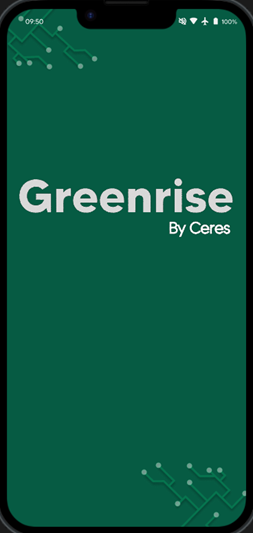
\includegraphics[scale=1]{Illustrations/Picture1.png}
\SourceOrNote{Autoria Própria (2024)}
\end{figure}

Foi criada uma Splash screen (tela de abertura) sem botões e apenas uma animação do logotipo do projeto e um leve delay para a tela seguinte.

\begin{figure}[!h]
\centering
\caption{Tela de login}
\label{fig:picture2}
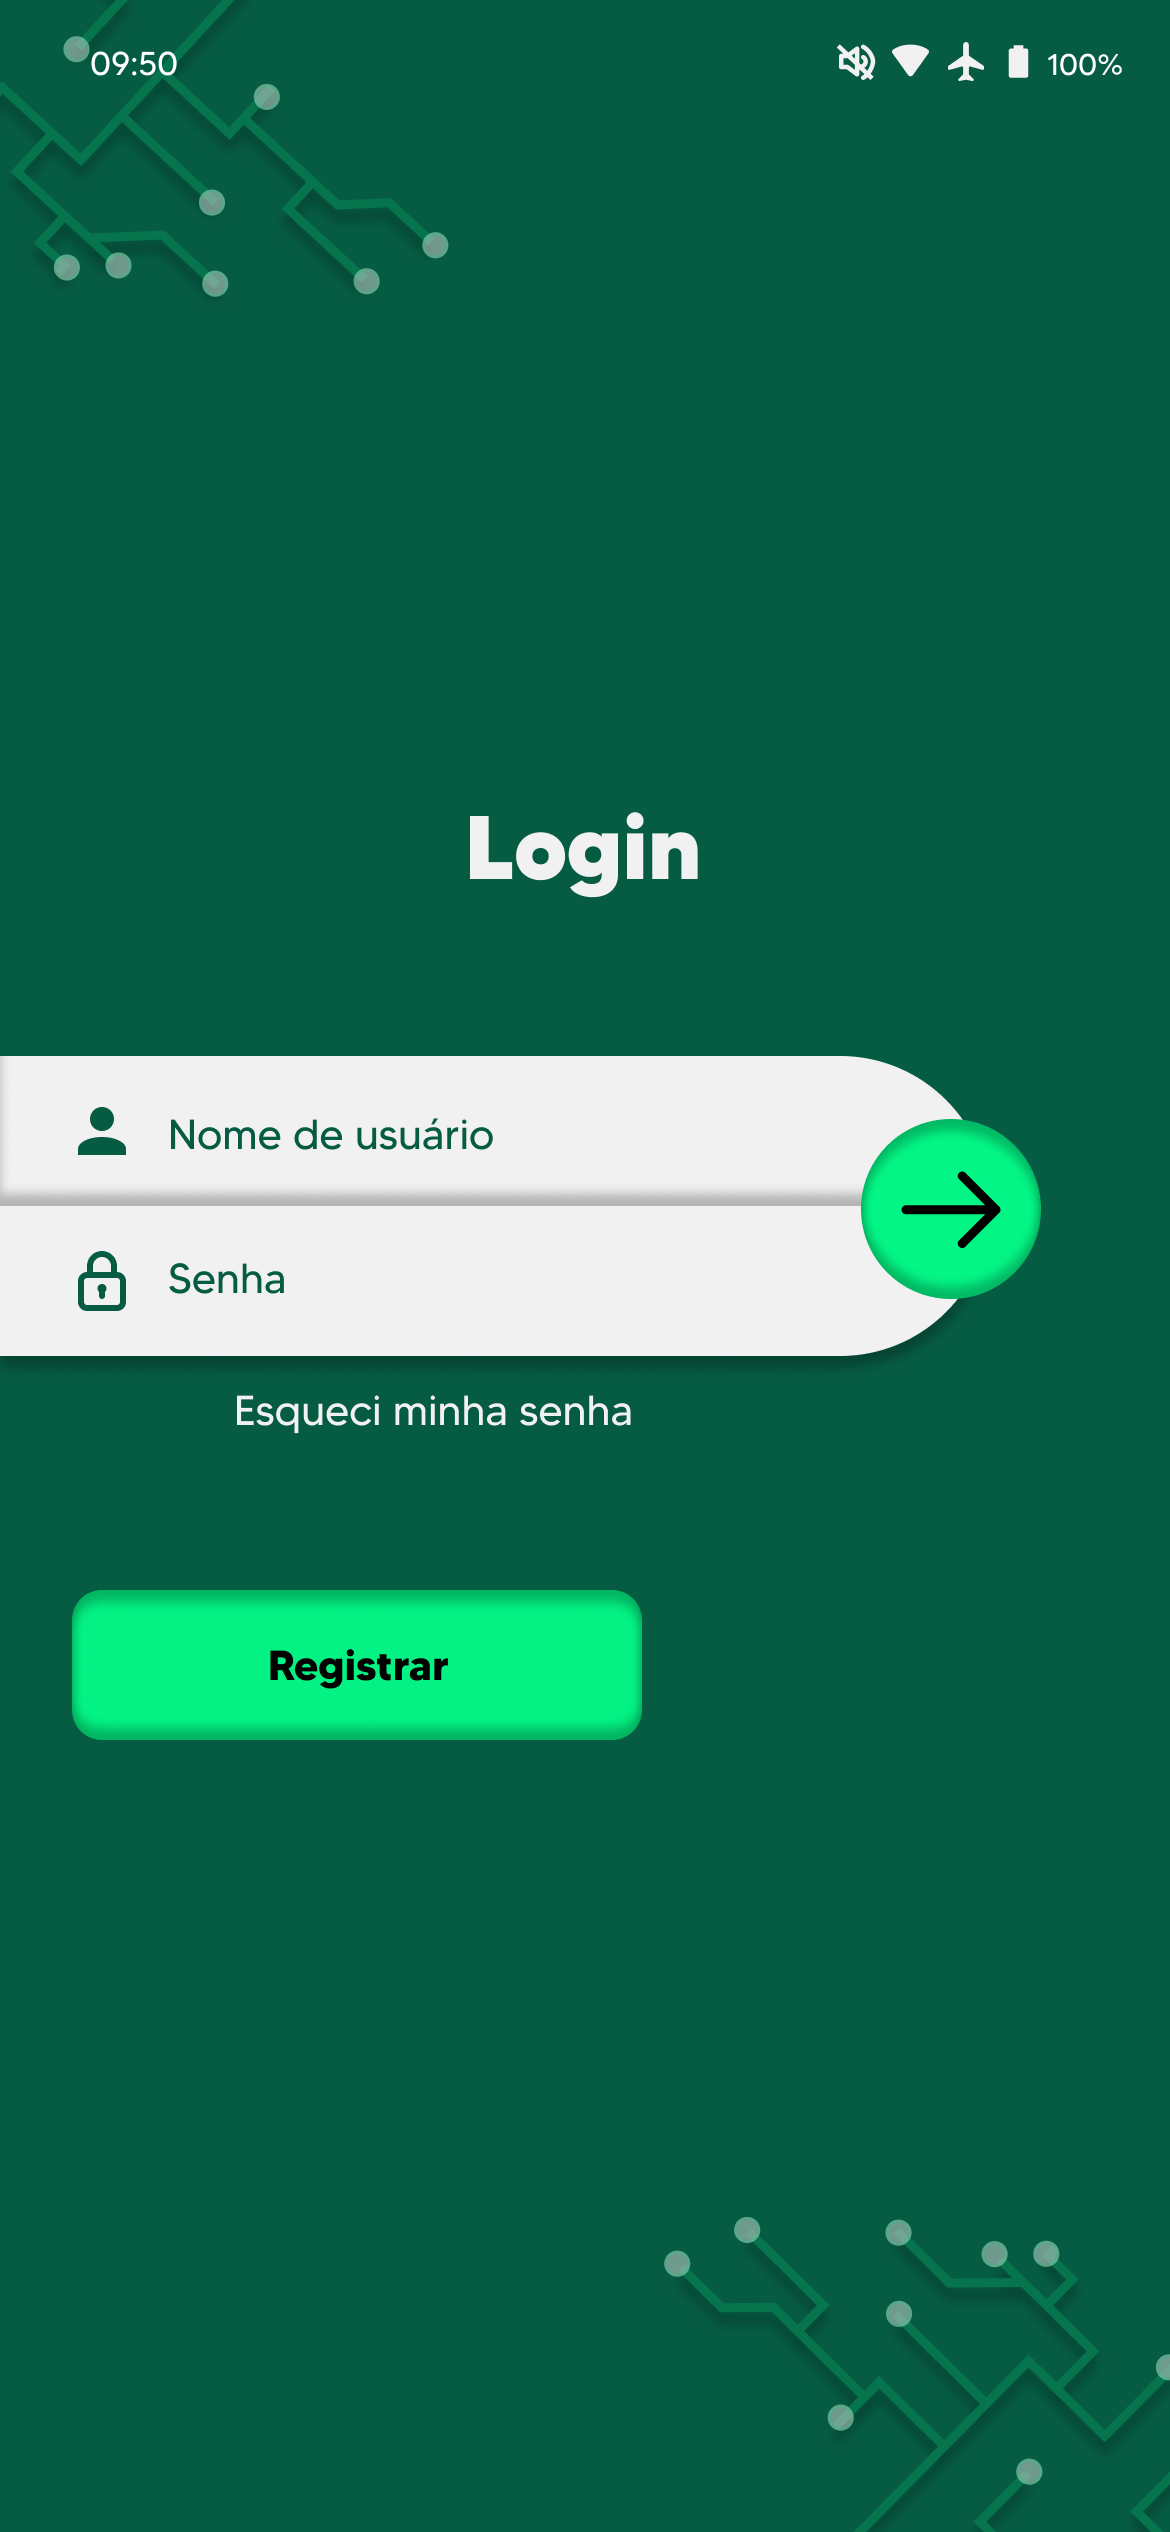
\includegraphics[scale=0.3]{Illustrations/Picture2.png}
\SourceOrNote{Autoria Própria (2024)}
\end{figure}
  
Após a tela de abertura temos a tela de login, onde o usuário deve inserir o usuário cadastrado e a senha nos campos designados. Caso tenha esquecido a senha, o sistema oferece ao usuário a opção de recuperação da mesma. Se o usuário não estiver cadastrado, ele deve clicar em “Registrar”, onde será encaminhado para a tela de registro.

\begin{figure}[!h]
\centering
\caption{Tela de registro}
\label{fig:picture3}
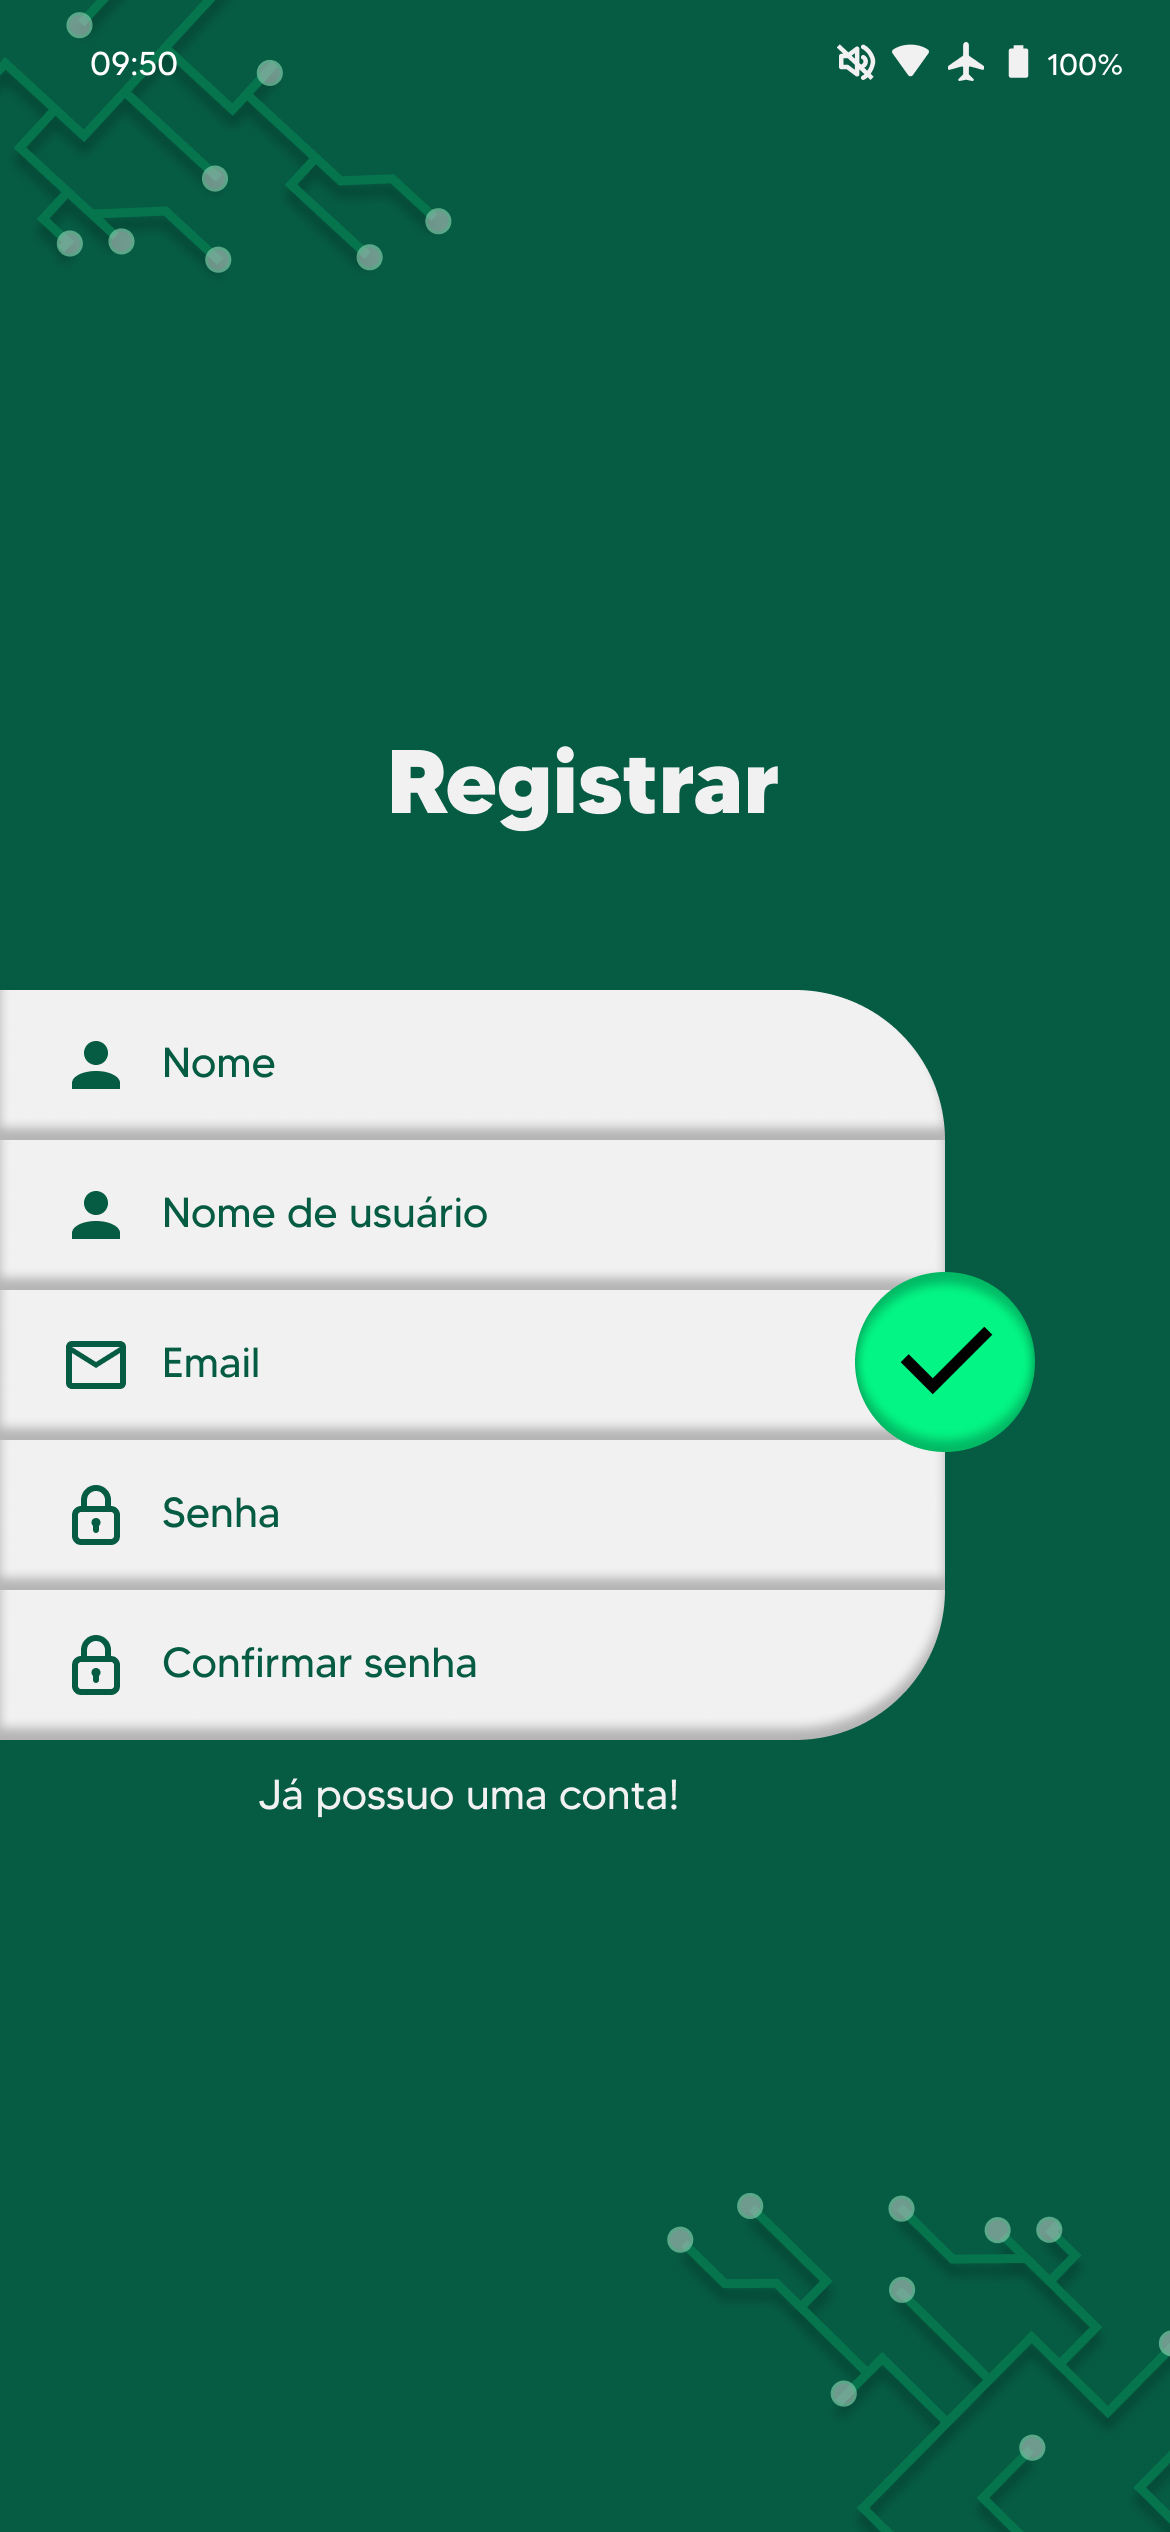
\includegraphics[scale=0.3]{Illustrations/Picture3.png}
\SourceOrNote{Autoria Própria (2024)}
\end{figure}

Caso o usuário precise se cadastrar ele será encaminhado para tela de registro. Para se registrar basta preencher os campos com seu nome completo, um nome de usuário, email, criar uma senha e confirmar a senha criada. Logo após, basta criar no ícone de confirmação para entrar no aplicativo.

\begin{figure}[!h]
\centering
\caption{Tela de boas-vindas}
\label{fig:picture4}
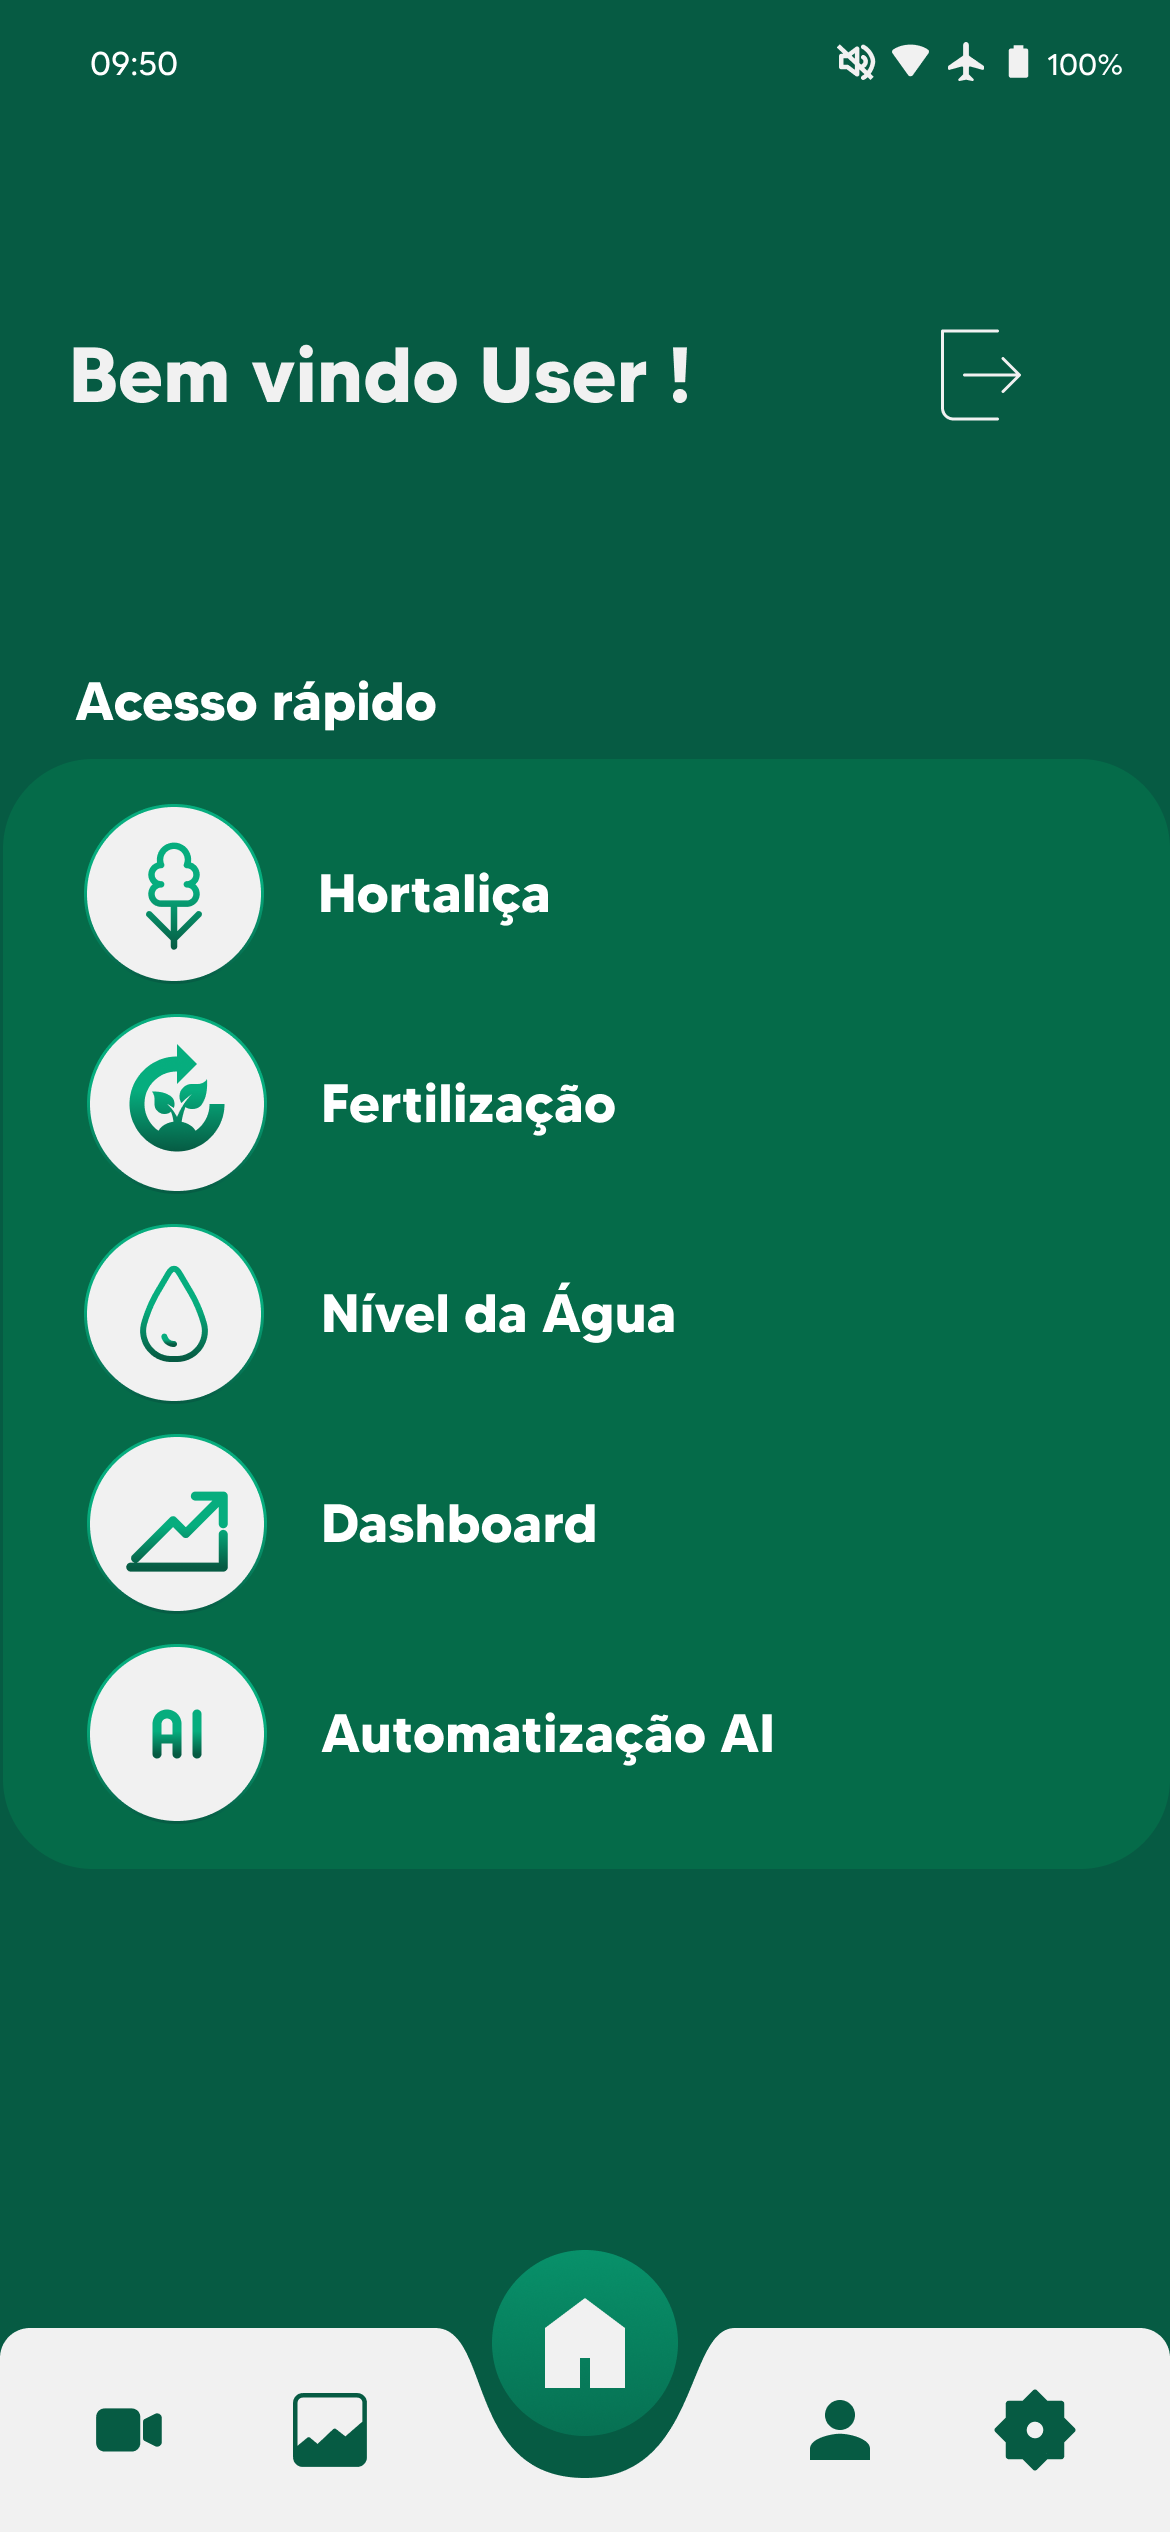
\includegraphics[scale=0.2]{Illustrations/Picture4.png}
\SourceOrNote{Autoria Própria (2024)}
\end{figure}
  
Ao centro da tela de boas-vindas são apresentados ícones de acesso rápido para os menus descritos de câmera em tempo real, hortaliça, fertilização, nível da água, dashboard e automatização AI. Na barra inferior temos o menu interativo do tipo carroussels e interações (da esquerda para a direita) para acesso às telas de câmera em tempo real, dashboards, página inicial, configurações do usuário e configuração do aplicativo. No canto superior direito temos o botão de voltar (que retorna para a tela de login).

\begin{figure}[!h]
\centering
\caption{Tela de dashboards}
\label{fig:picture5}
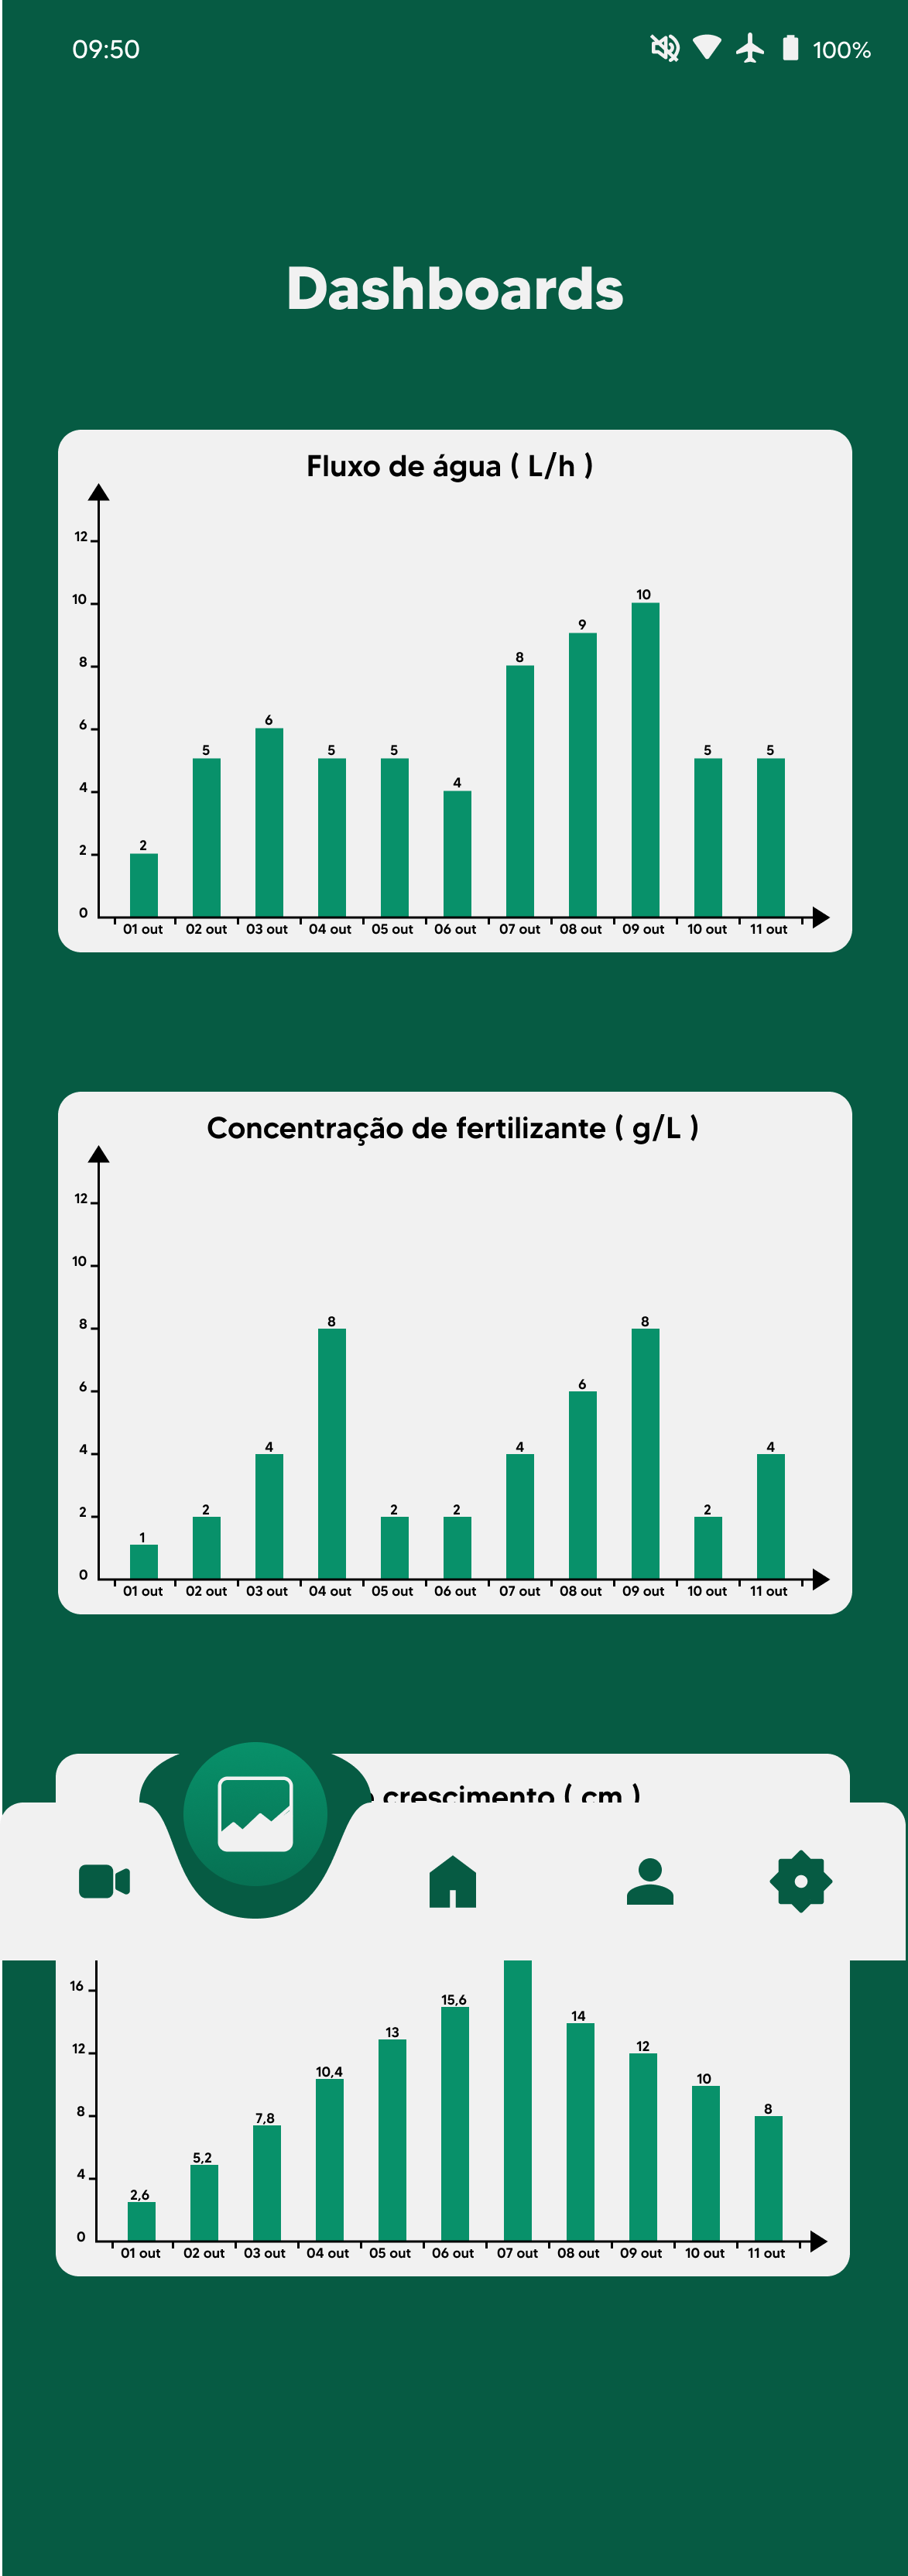
\includegraphics[scale=0.3]{Illustrations/Picture5.png}
\SourceOrNote{Autoria Própria (2024)}
\end{figure}

A tela de dashboards apresenta os dados históricos de fluxo de água, concentração de fertilizante e a taxa de crescimento da(s) cultura(s). A tela tem a opção de rolagem para exibição dos gráficos. Por sua vez, os gráficos são gerados automaticamente com base nos dados obtidos pelos sensores instalados na fazenda vertical.
\clearpage
\begin{figure}[!h]
\centering
\caption{Tela de configurações do aplicativo}
\label{fig:picture6}
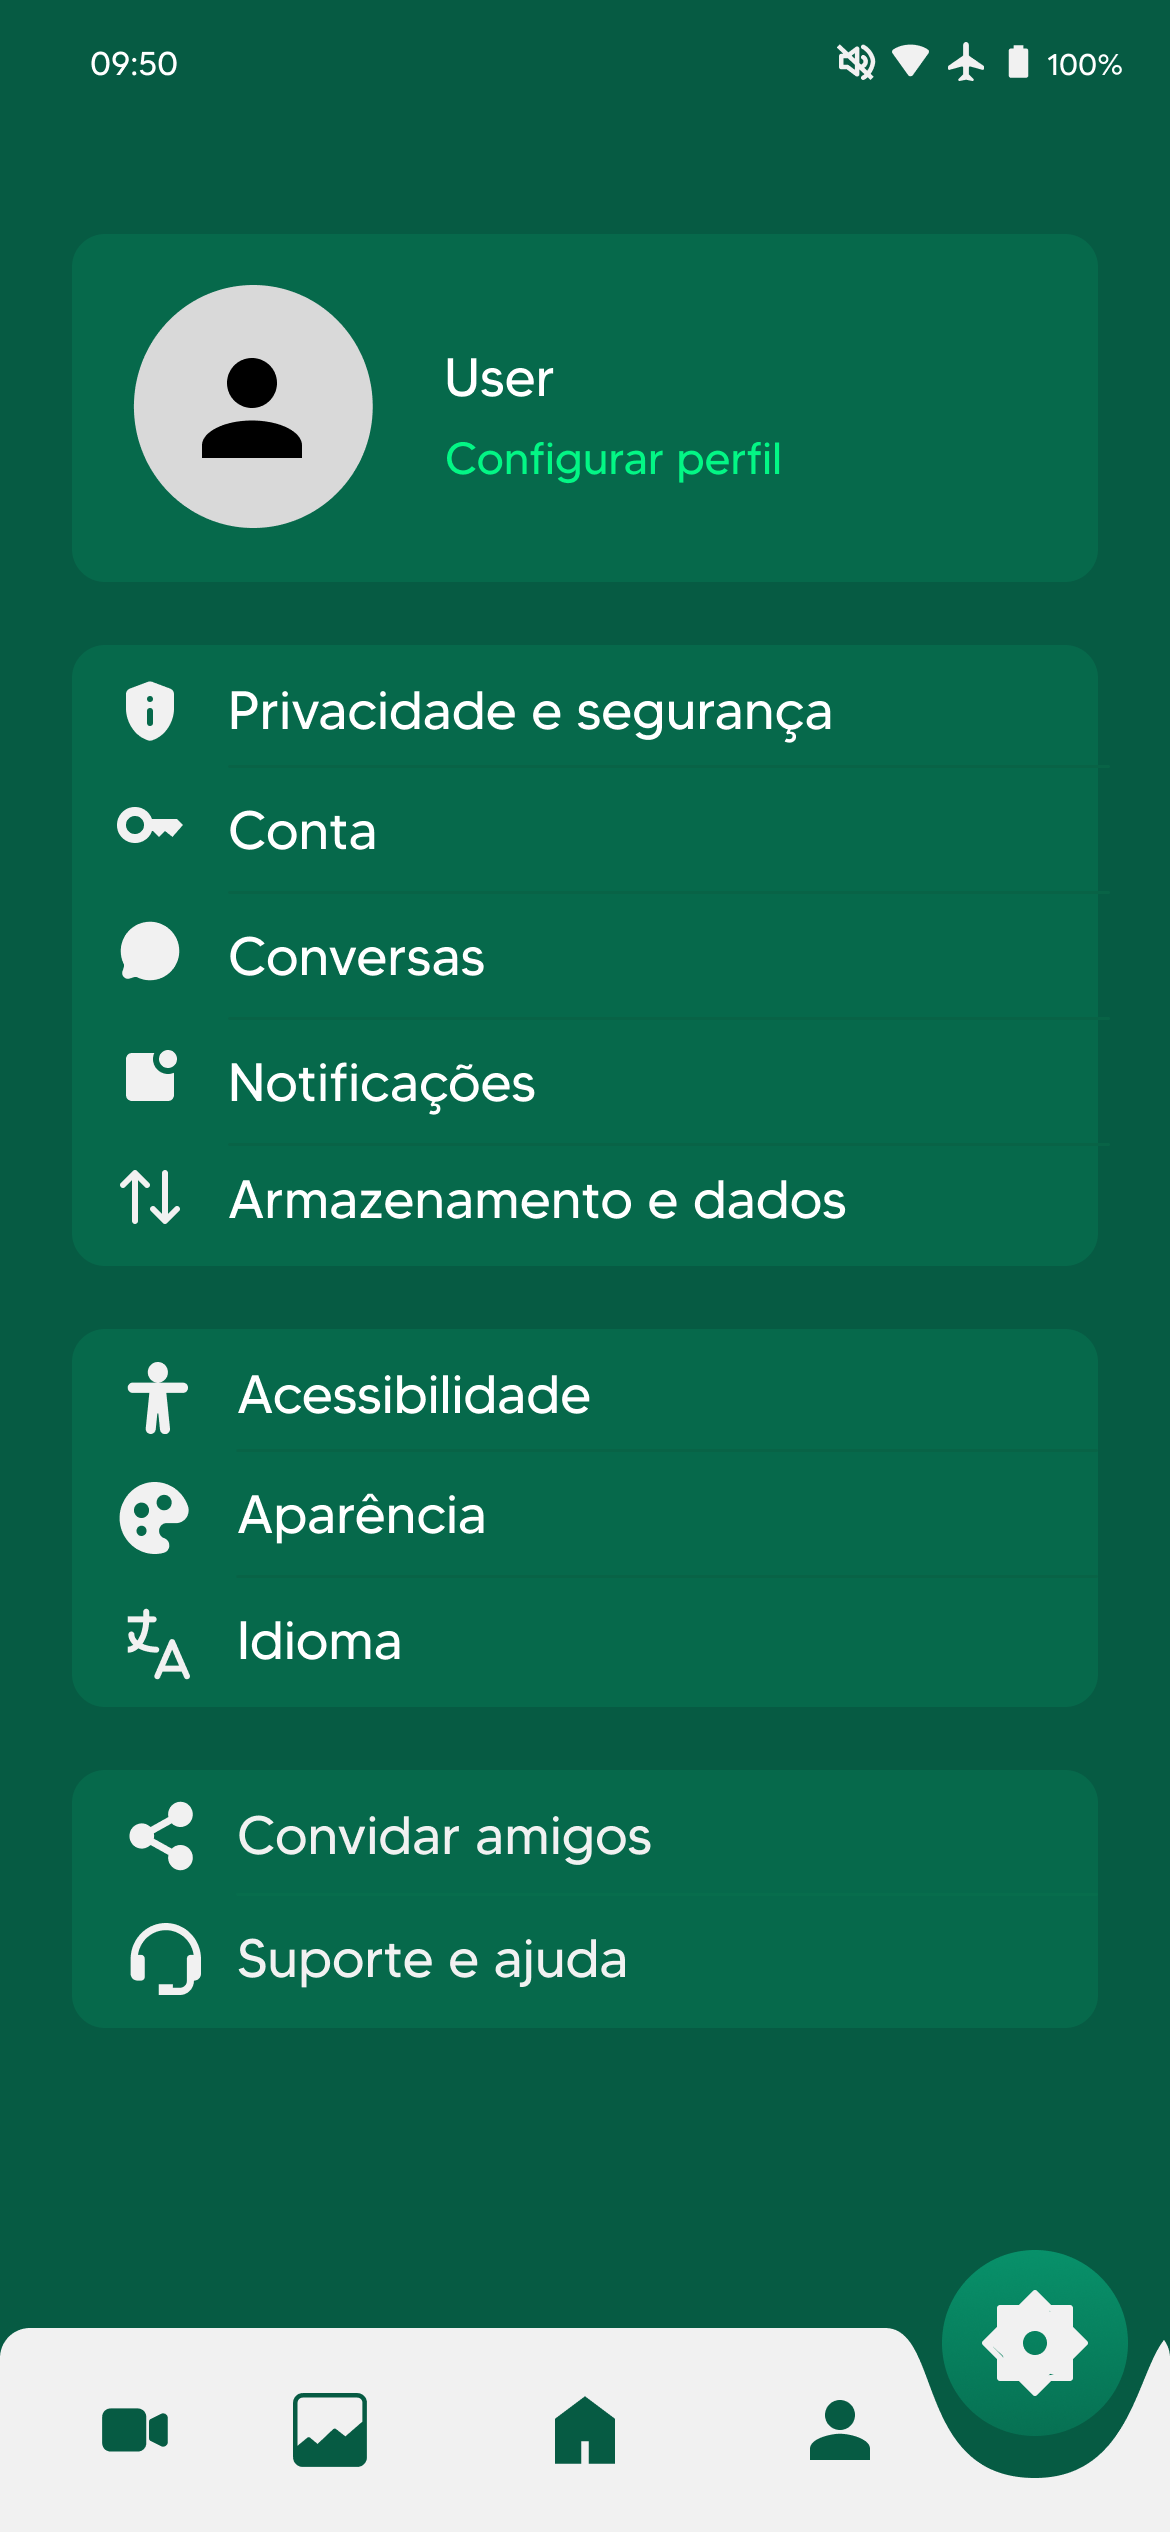
\includegraphics[scale=0.3]{Illustrations/Picture6.png}
\SourceOrNote{Autoria Própria (2024)}
\end{figure}

A tela de configurações do aplicativo é composta da imagem (editável) do usuário com atalho para configurações do perfil e botões de privacidade e segurança, conta, conversas, notificações, armazenamento e dados, acessibilidade, aparência, idioma, convidar amigos e suporte e ajuda.

\begin{figure}[!h]
\centering
\caption{Tela de câmeras}
\label{fig:picture7}
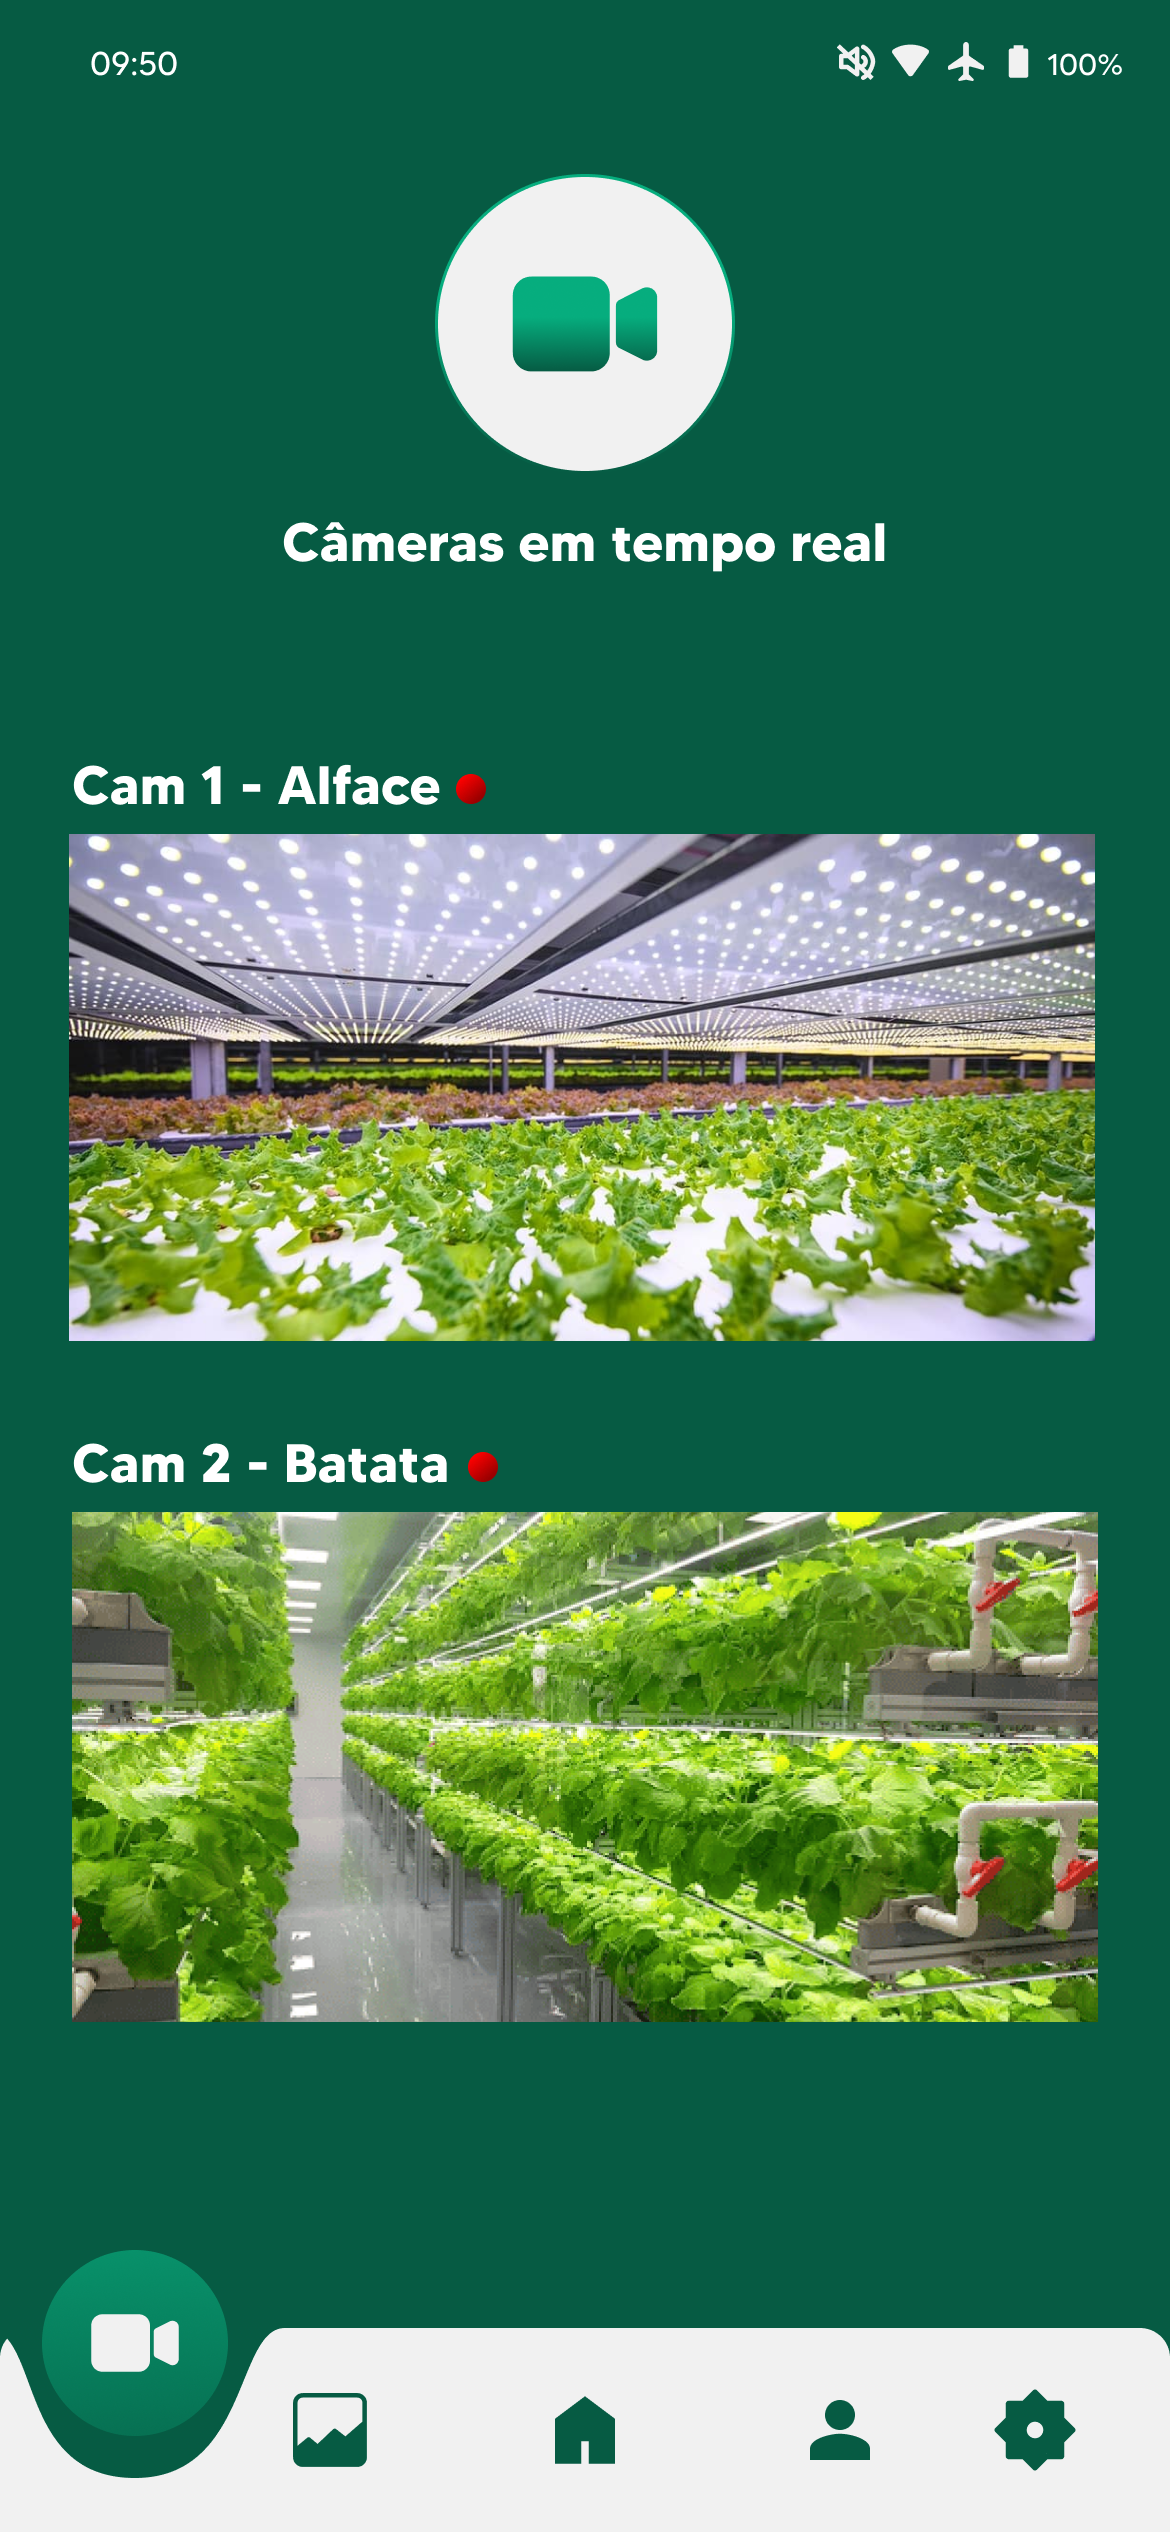
\includegraphics[scale=0.3]{Illustrations/Picture7.png}
\SourceOrNote{Autoria Própria (2024)}
\end{figure}
A tela de câmeras em tempo real contem um íconde decorativo no topo, ao centro. Ela exibe as imagens captadas pela(s) câmera(s) que acompanham a produção da fazenda vertical do usuário. A tela também apresenta a opção de rolagem da página caso tenha mais de uma câmera monitorando a produção da fazenda.

\begin{figure}[!h]
\centering
\caption{Tela de hortaliça}
\label{fig:picture8}

\includegraphics[scale=0.3]{Illustrations/Picture8.png}
\SourceOrNote{Autoria Própria (2024)}
\end{figure}
A tela de hortaliça é composta de um ícone decorativo no topo. Ao centro temos uma lista suspensa onde o usuário deve escolher o tipo de vegetal que será cultivado na fazenda vertical.

\begin{figure}[!h]
\centering
\caption{Tela de fertilização}
\label{fig:picture9}
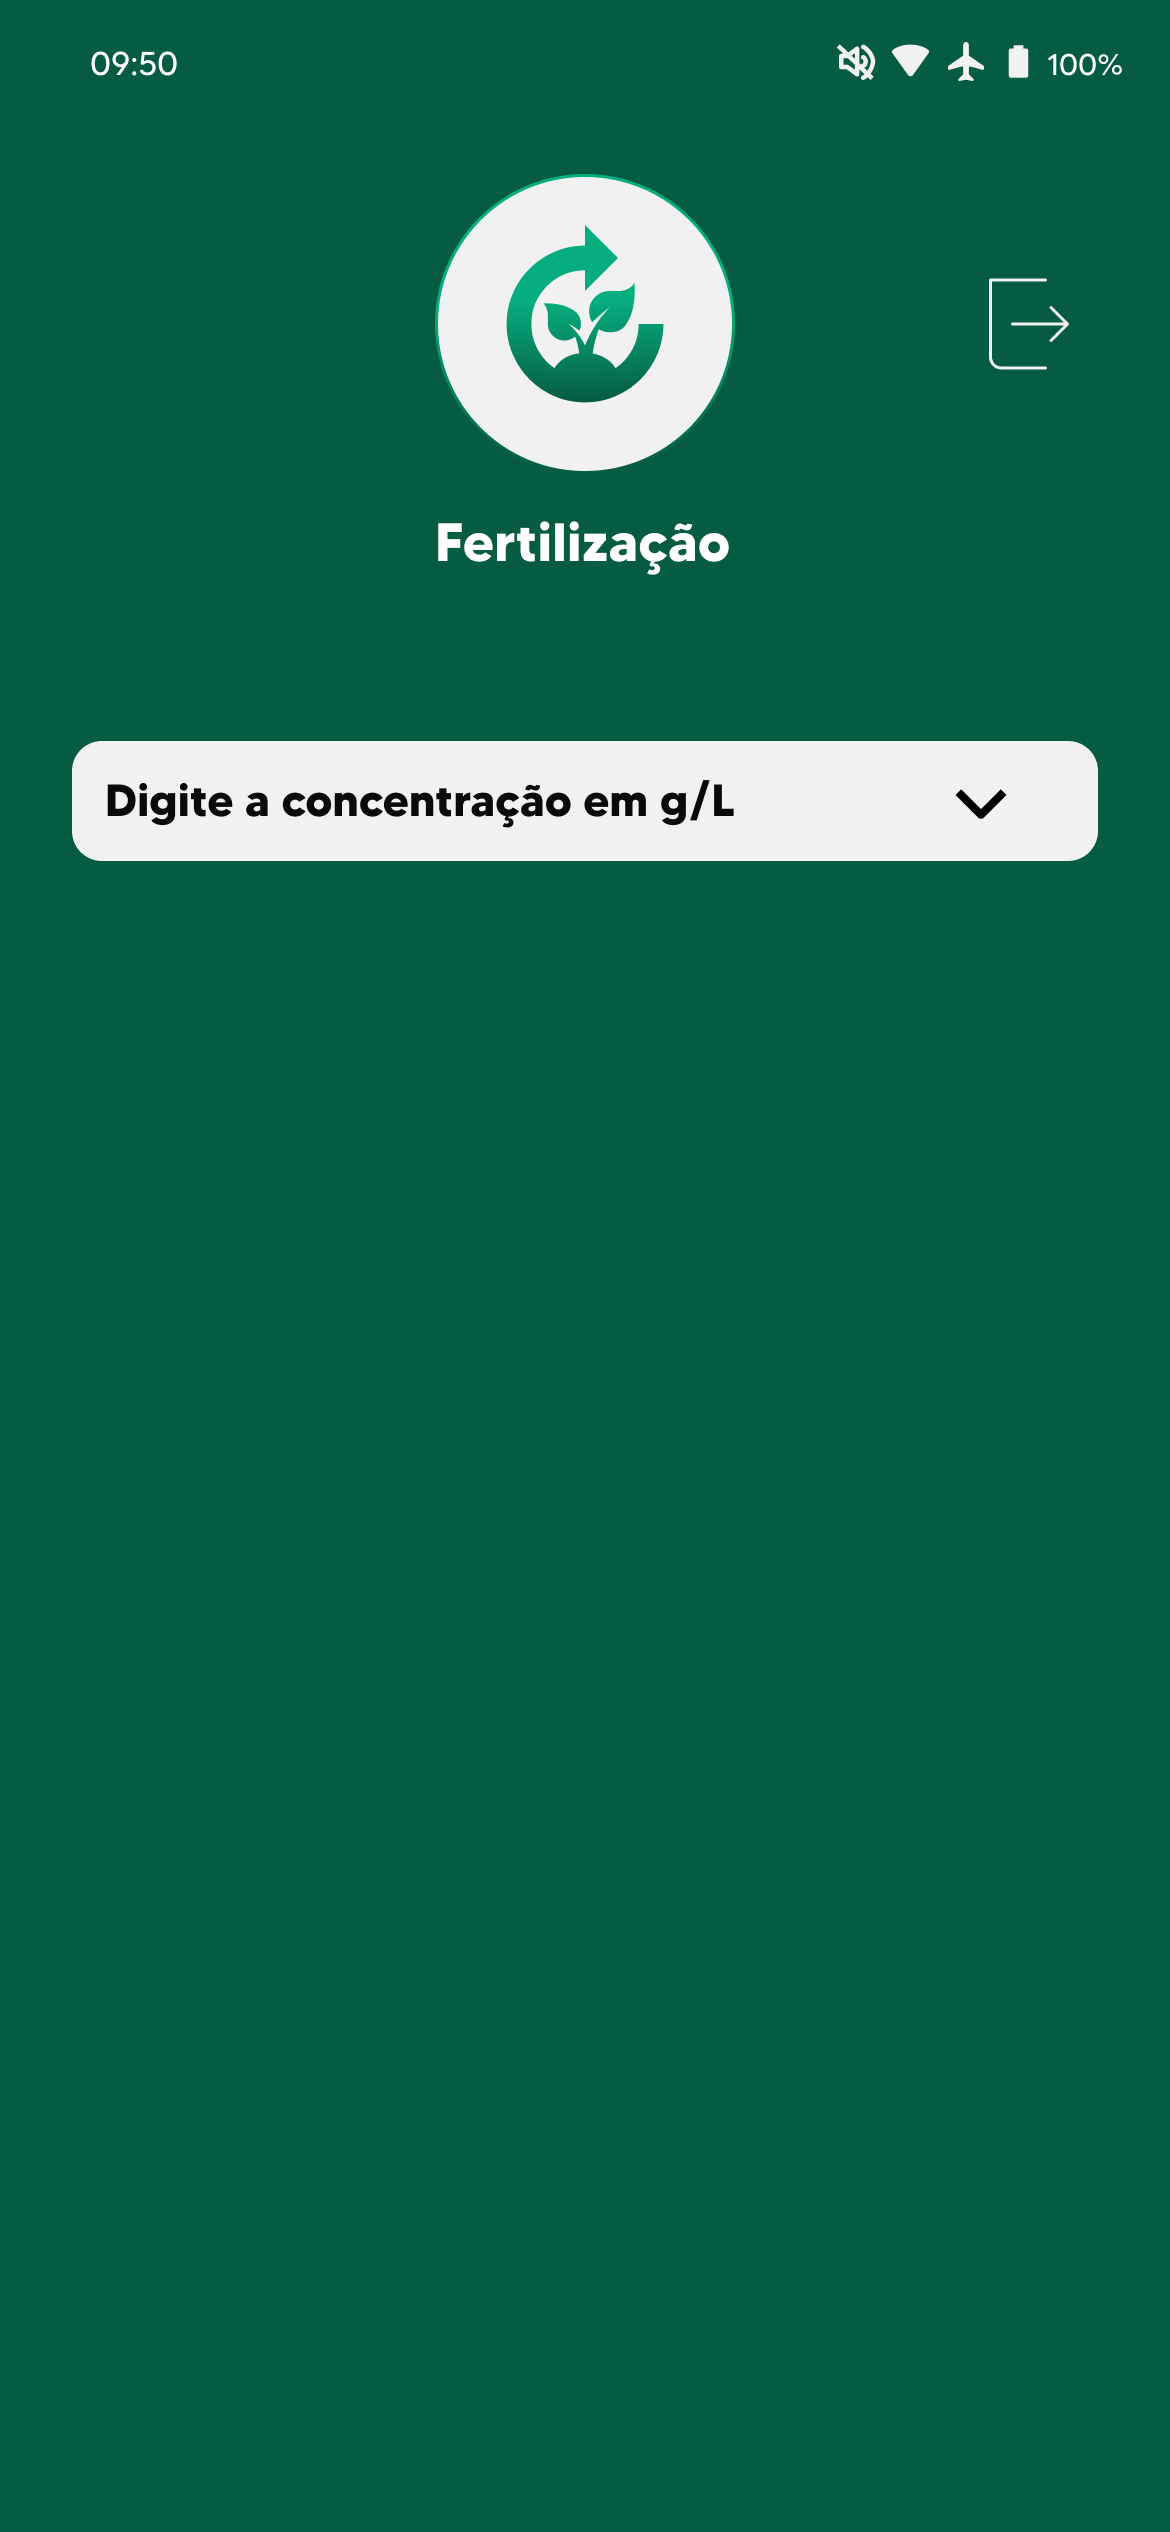
\includegraphics[scale=0.3]{Illustrations/Picture9.png}
\SourceOrNote{Autoria Própria (2024)}
\end{figure}
A tela de fertilização contém um ícone decorativo centralizado, acima. Ao centro da tela temos um campo onde o usuário deverá digitar a concentração do fertilizante em gramas por litro.
\begin{figure}[!h]
\centering
\caption{Tela de nível da água}
\label{fig:picture10}
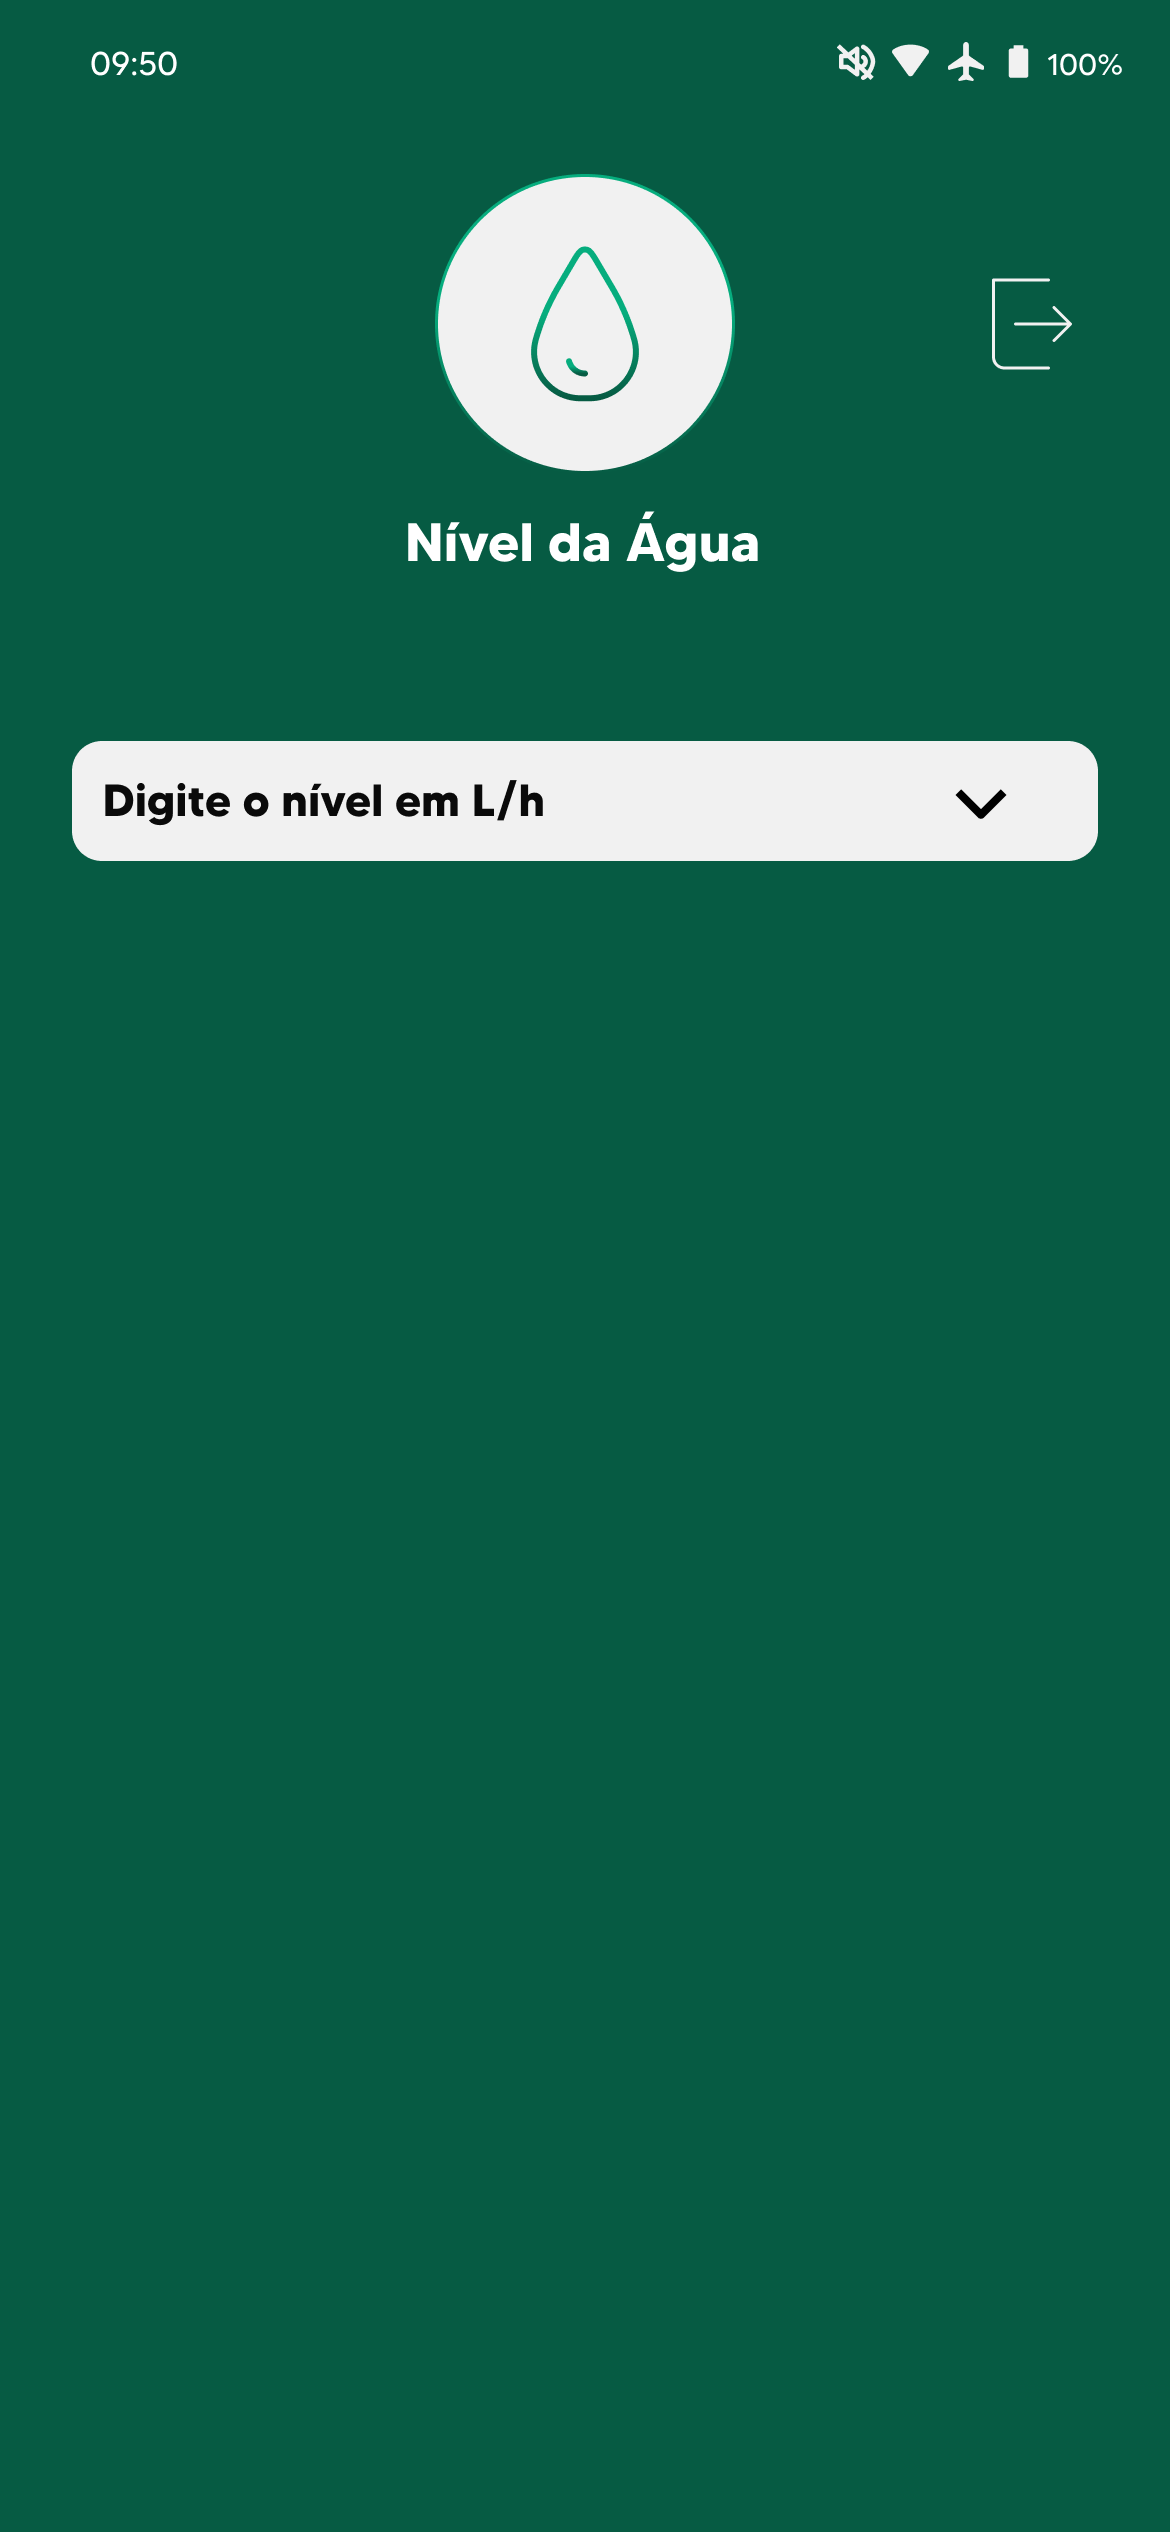
\includegraphics[scale=0.3]{Illustrations/Picture10.png}
\SourceOrNote{Autoria Própria (2024)}
\end{figure}
A tela de nível da água contém um ícone decorativo centralizado no topo. Nesta tela o usuário deverá digitar a pressão da água (em litros por hora) que passa pelo sistema de fazenda vertical.
\clearpage
\begin{figure}[!h]
\centering
\caption{Tela de automatização AI}
\label{fig:picture11}
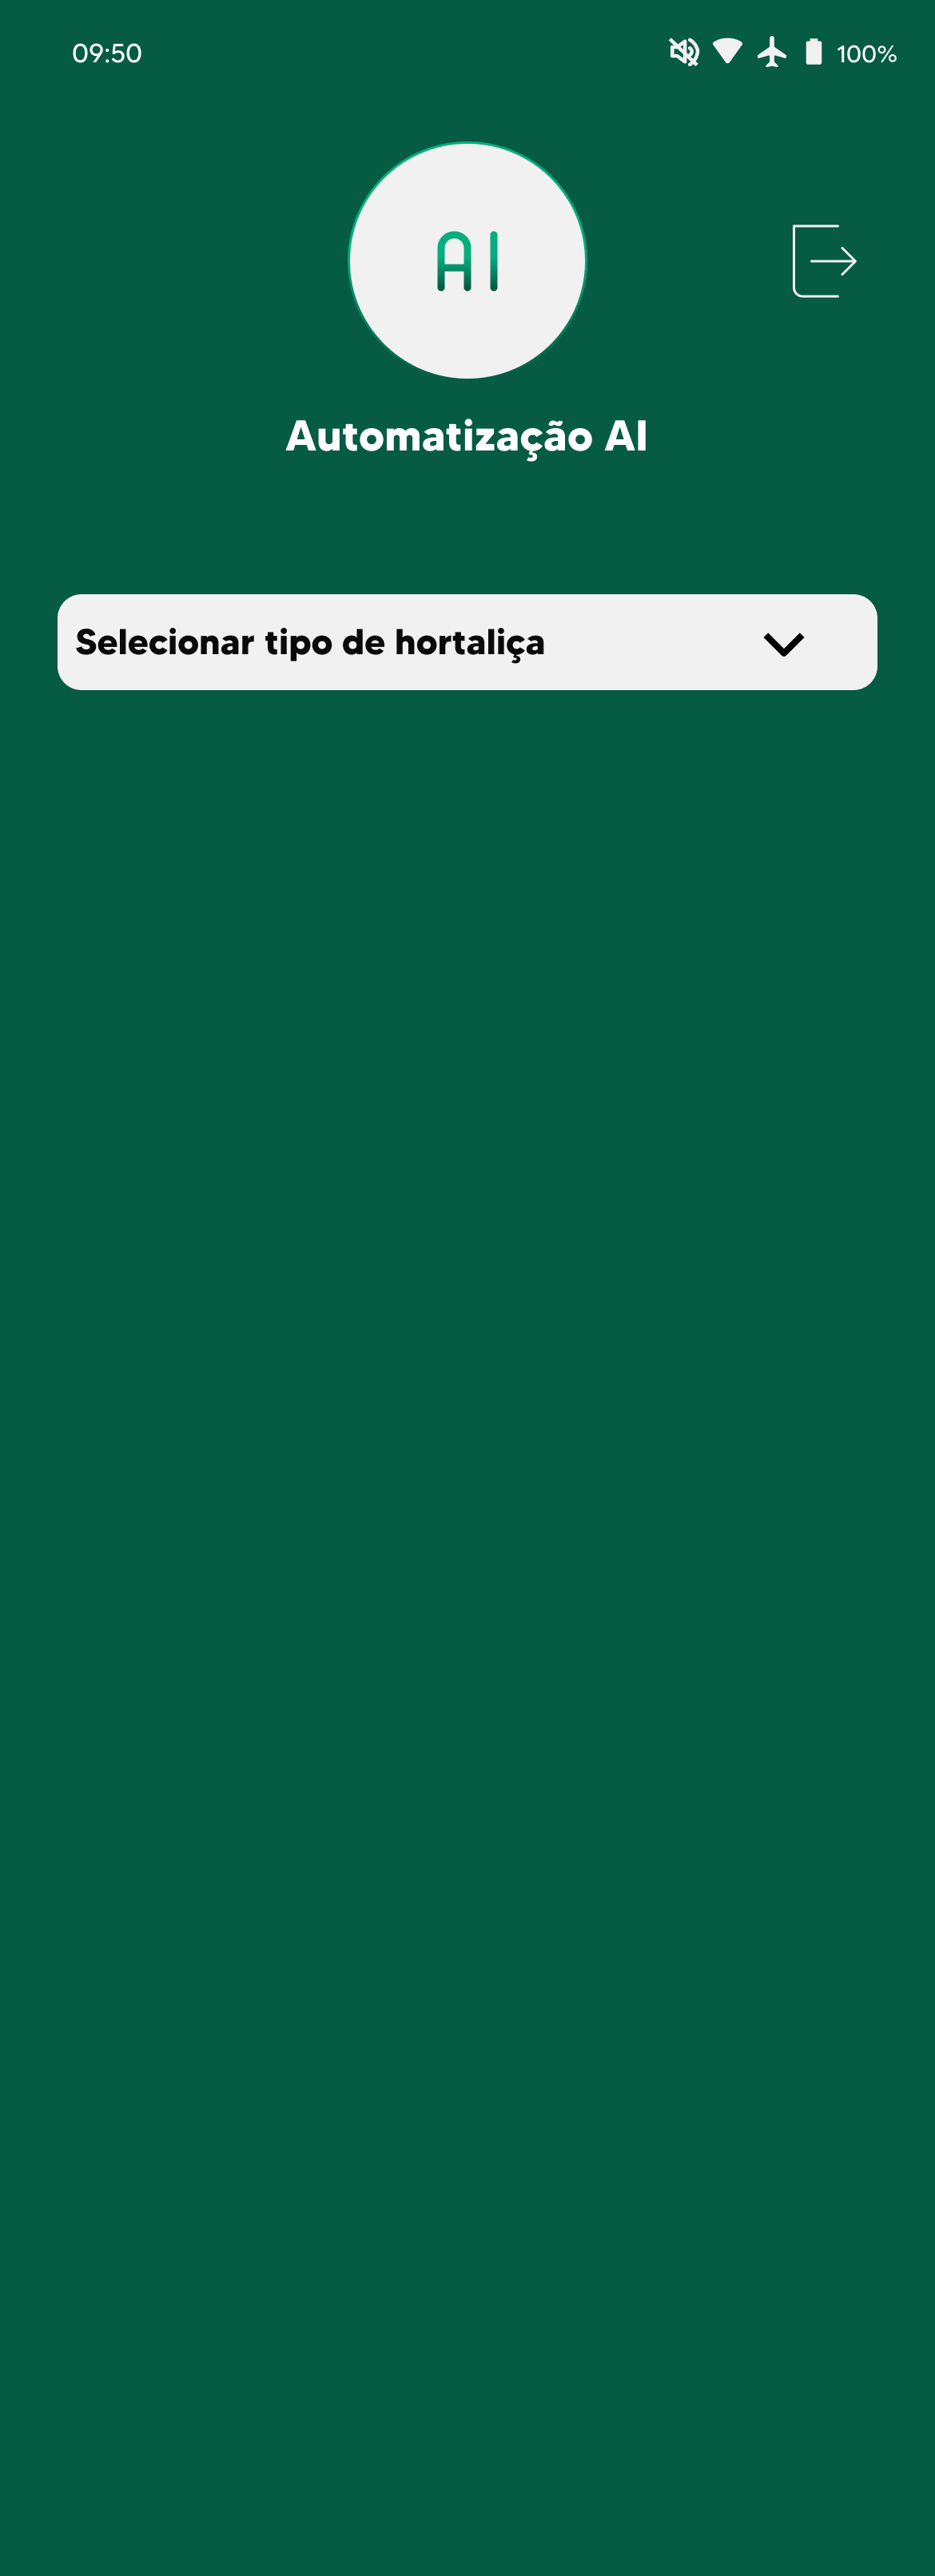
\includegraphics[scale=0.2]{Illustrations/Picture11.png}
\SourceOrNote{Autoria Própria (2024)}
\end{figure}
A tela de automatização AI permite que o usuário escolha se deseja que a rede neural tenha total controle da fazenda vertical e sua produção. Esta tela também oferece a opção de o usuário controlar pessoalmente alguns parâmetros (controle semi-autônomo) ou controlar todas as configurações (controle manual).
            
\subsection*{DIAGRAMA DE BANCO DE DADOS}

A modelagem do banco de dados foi realizada no software Brmodelo. A modelagem de dados define como o sistema vai trabalhar o fluxo de dados e como estes dados serão utilizados. No contexto deste estudo, os dados desempenham um papel central no processo de tomada de decisão, seja por meio de algoritmos de inteligência artificial, seja por intervenção direta do usuário.

\subsection*{1. Modelo conceitual}

O modelo conceitual foi desenvolvido para representar o banco de dados com foco em entidades, atributos e os relacionamentos entre eles. A seguir é apresentada a estrutura conceitual do banco de dados proposto.

\clearpage
\begin{figure}[!h]
\centering
\caption{Modelo conceitual}
\label{fig:picture14}
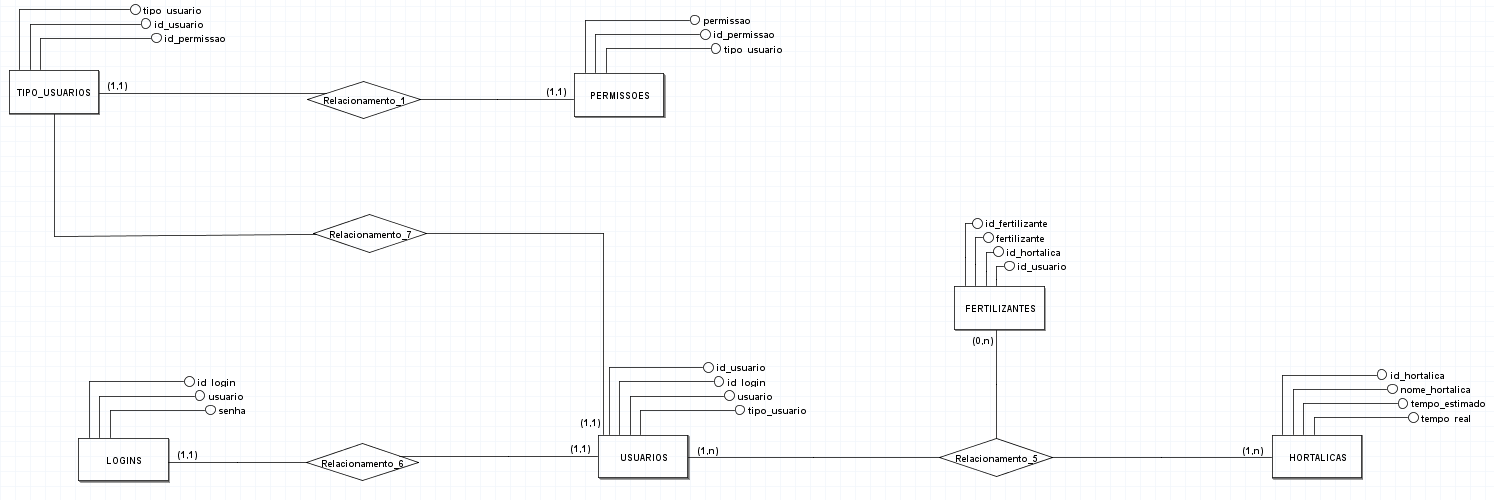
\includegraphics[scale=0.4]{Illustrations/modelo conceitual.png}
\SourceOrNote{Autoria Própria (2024)}
\end{figure}

Foram mapeadas seis entidades (colunas) diferentes, vinte e um atributos e quatro relacionamentos.

\subsection*{2. Modelo lógico}

O modelo lógico detalha o banco de dados em termos de atributos específicos, incluindo tipo de dado, obrigatoriedade e unicidade. 

\begin{figure}[!h]
\centering
\caption{Modelo clógico}
\label{fig:picture15}
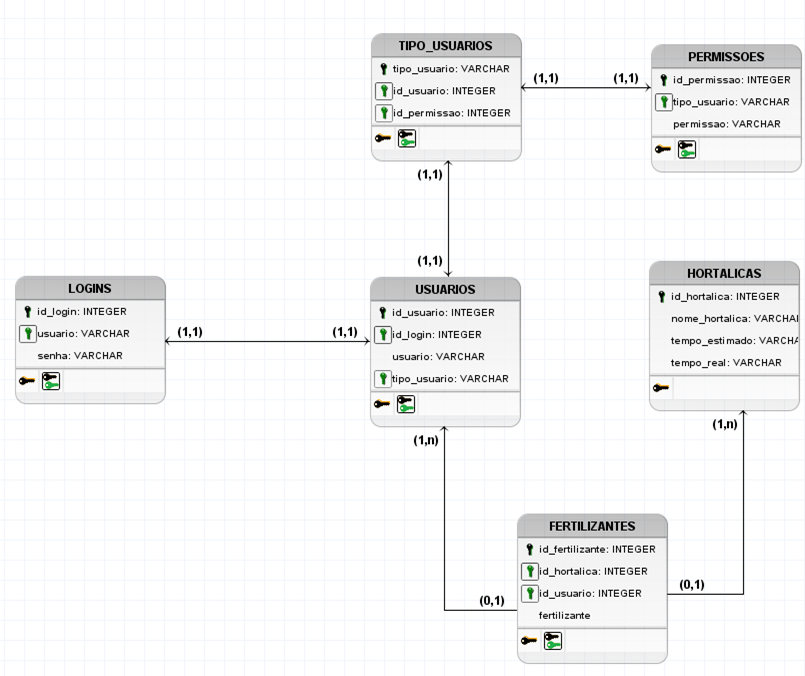
\includegraphics[scale=0.8]{Illustrations/modelo logico.png}
\SourceOrNote{Autoria Própria (2024)}
\end{figure}

Nesta fase foram identificadas seis chaves primárias e oito chaves estrangeiras. O modelo inclui ainda dez atributos do tipo INTEGER e onze atributos do tipo VARCHAR que representam dados numéricos e textuais, respectivamente. Realizamos uma revisão para garantir que todas as entidades tivessem chaves primárias entre seus atributos, garantindo a unicidade do banco de dados. Além disso, o sistema contará com diversas chaves estrangeiras que realizem corretamente o relacionamento entre as entidades envolvidas.

\subsection*{DIAGRAMA DE SISTEMA}

A diagramação do sistema foi realizada considerando pontos-chave para a estrutura do software. Primeiramente, à partir do celular do usuário (a), os dados serão enviados à um roteador conectado à internet (b). Paralelamente na fazenda vertical, o(s) sensor(es) conectado(s) por Arduino (c) enviarão seus resultados também para internet via roteador. Na sequência os dados serão armazenados (d) em nuvem utilizando o sistema Oracle Cloud (f). Utilizando o sistema GenAI Oracle os dados são analisados (e) e uma resposta é enviada ao celular do usuário, apresentando os valores ideais de operação identificados pelo algoritmo. Além disso, também conectado ao Oracle Cloud teremos um PC emitindo relatórios em tempo real sobre o banco de dados e informações relevantes sobre o status da operação (g).

\begin{figure}[!h]
\centering
\caption{Diagrama de sistema}
\label{fig:picture16}
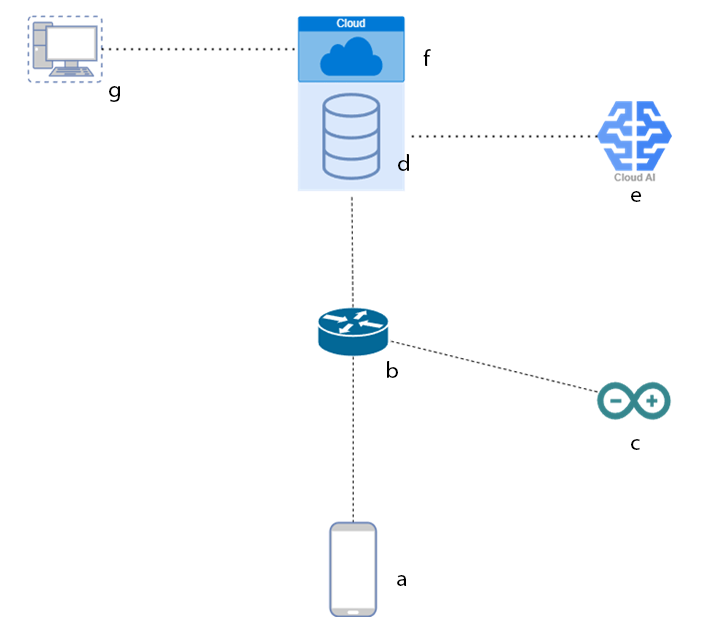
\includegraphics[scale=0.8]{Illustrations/diagrama de sistema 2.png}
\SourceOrNote{Autoria Própria (2024)}
\end{figure}
Esta é uma etapa crítica pois uma das bases do trabalho é a utilização da rede neural para o desenvolvimento do projeto. Além disso o sistema de armazenamento em nuvem e backup garantem a integridade dos dados.
\subsection*{ANÁLISE DO PROJETO (CANVAS)}

A análise do projeto foi realizada por meio do Canvas disponível no site do Sebrae. A avaliação foi realizada levando em consideração os dados levantados no presente projeto e aspectos potenciais da proposta.

\clearpage
\begin{figure}[!h]
\centering
\caption{Diagrama de sistema}
\label{fig:picture17}
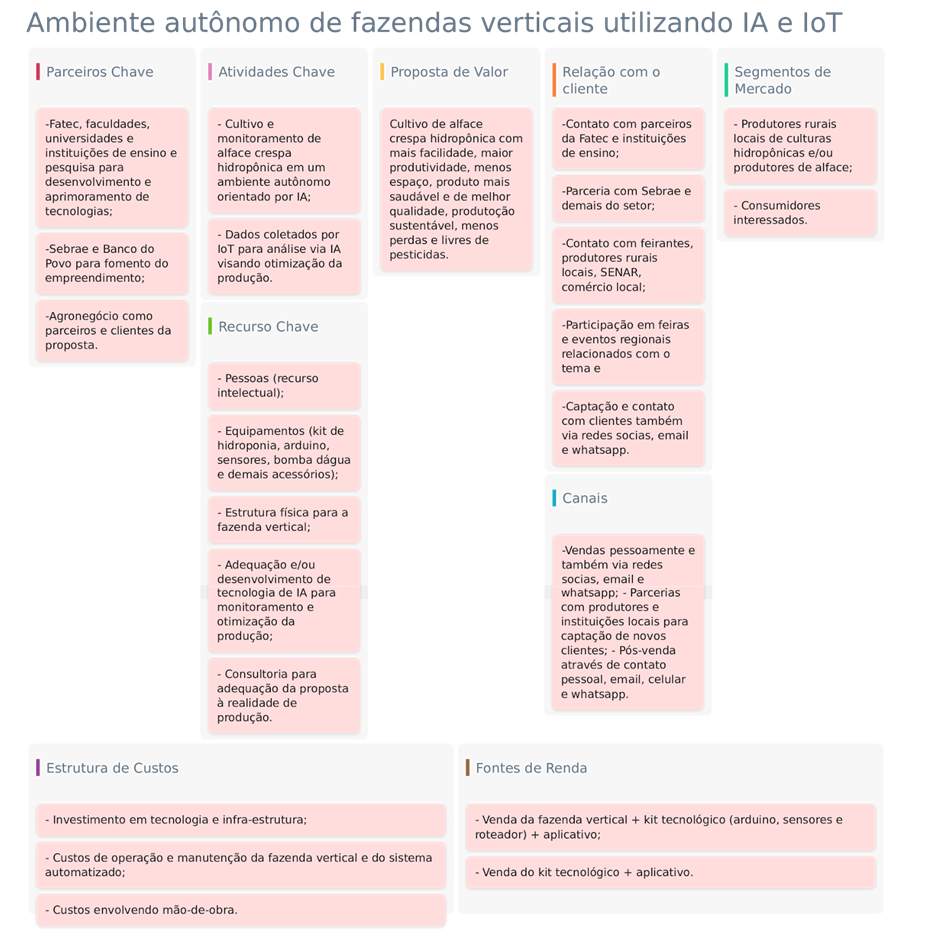
\includegraphics[scale=0.8]{Illustrations/CANVAS.png}
\SourceOrNote{Autoria Própria (2024)}
\end{figure}

Com o Canvas é possível observar o caráter empreendedor do projeto. Além disso observamos diversas oportunidades e pontos de melhoria que impactam na viabilidade do projeto como empreendimento.

\subsection*{PLATAFORMA WEB (APEX)}

O sistema proposto foi elaborado na plataforma web em um sistema low code. Todo o sistema é responsivo, podendo ser exibido tanto em smartphones quanto em tablets ou computadores. A plataforma apresenta por padrão um banco de dados em nuvem, garantindo assim a integridade dos dados. 
\clearpage
\begin{figure}[!h]
\centering
\caption{Tela de login}
\label{fig:picture18}
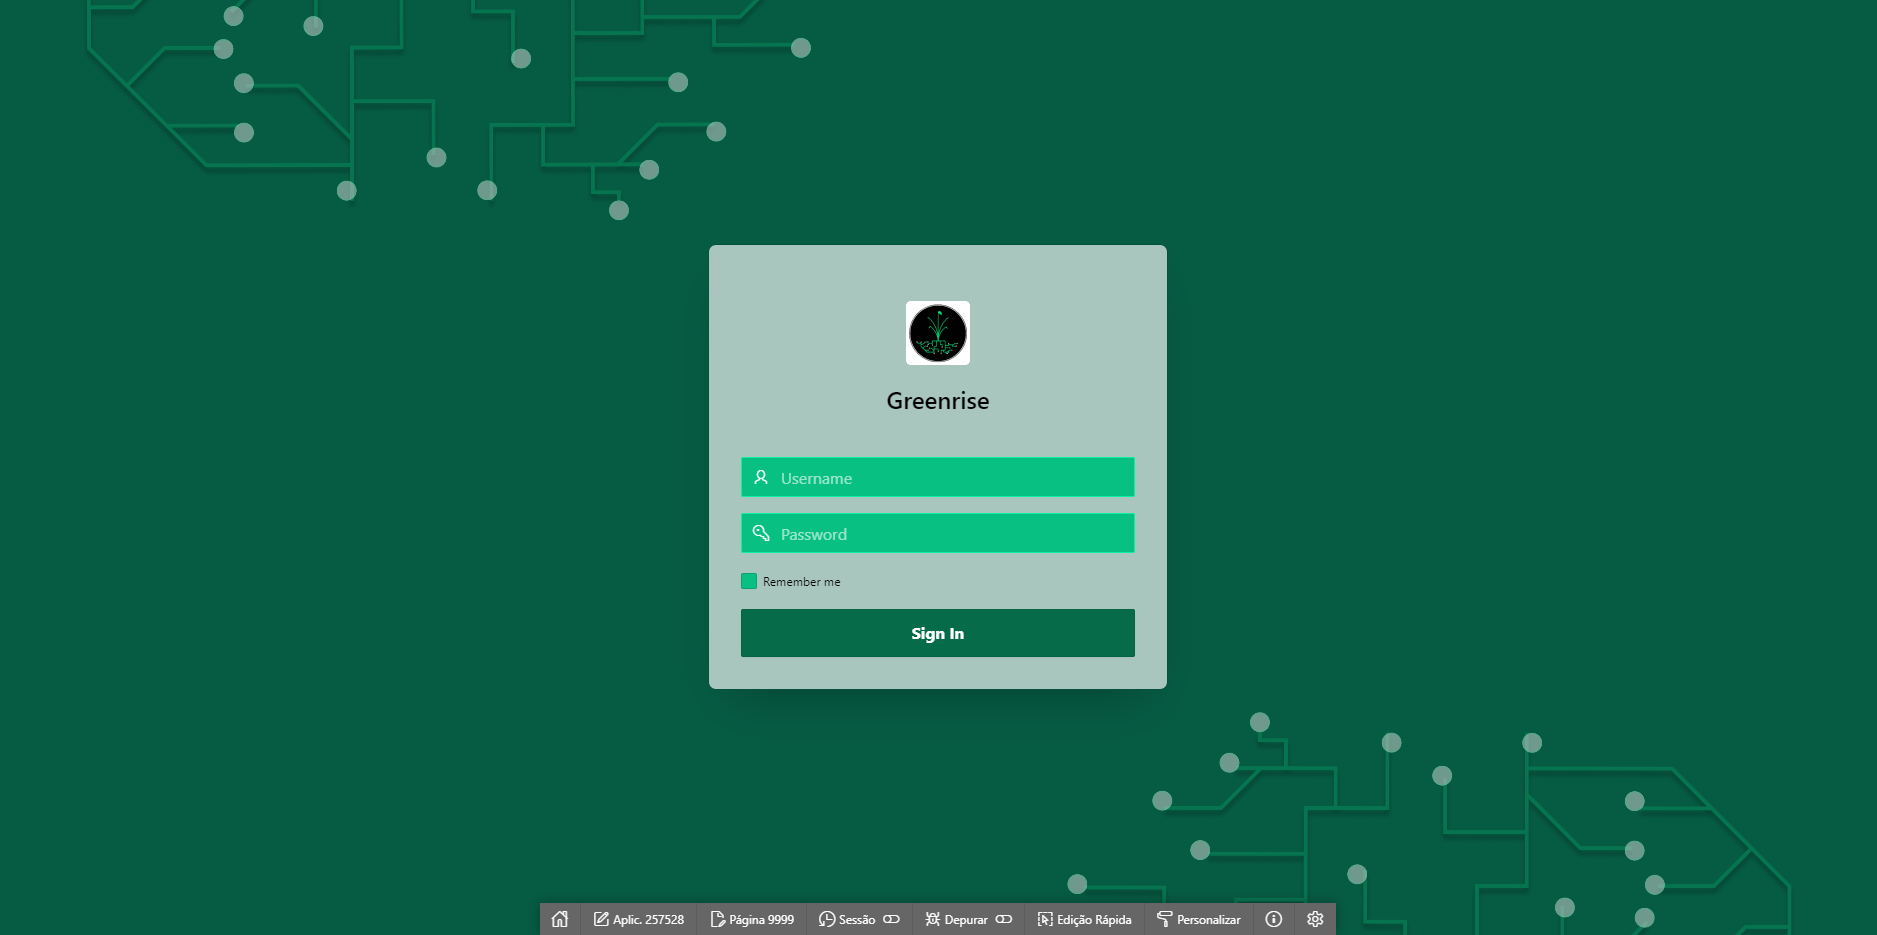
\includegraphics[scale=0.2]{Illustrations/Tela_login.png}
\SourceOrNote{Autoria Própria (2024)}
\end{figure}
Seguindo as premissas pré-estabelecidas o sistema foi elaborado com uma tela de login (onde o usuário preenche com seu nome e senha) para acesso ao sistema. Esta também é uma forma de garantir a segurança do acesso ao sistema.
\begin{figure}[!h]
\centering
\caption{Tela inicial}
\label{fig:picture19}
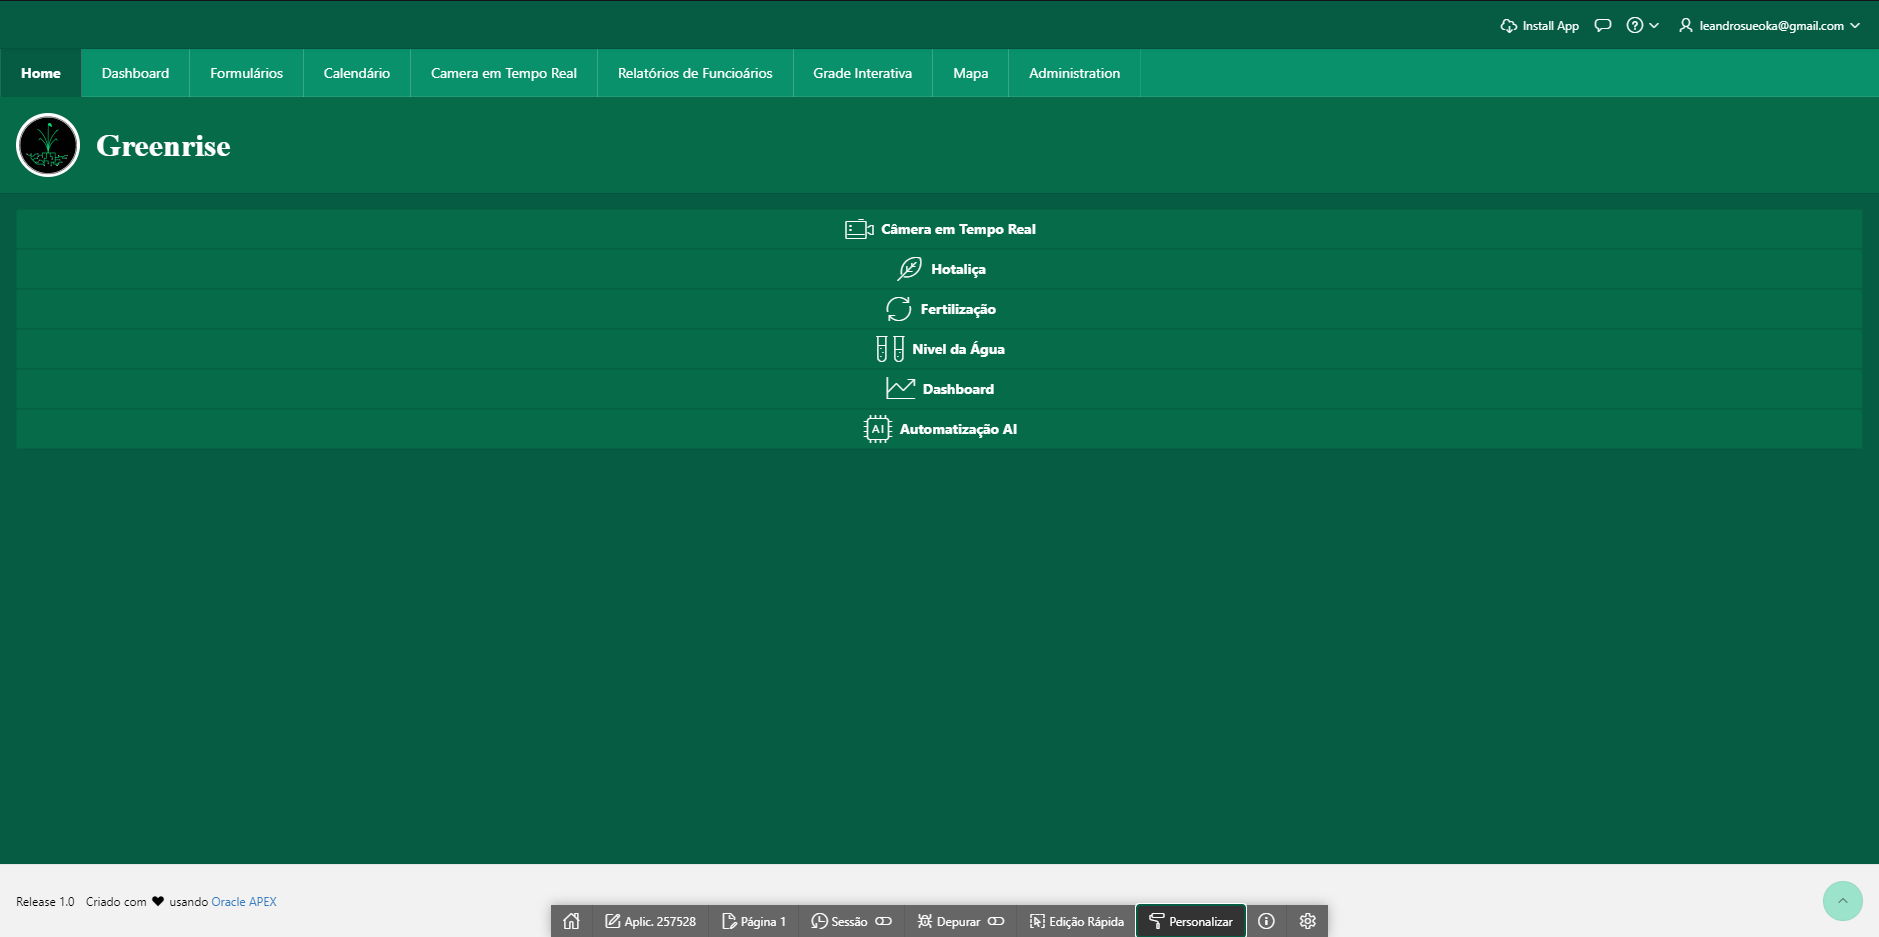
\includegraphics[scale=0.2]{Illustrations/Tela_home.png}
\SourceOrNote{Autoria Própria (2024)}
\end{figure}

Na tela inicial são apresentados os dados cadastrados (tipo de hortaliça, fertilizante, concentração e fluxo de água). Na barra superior temos o menu onde é possível navegar pelas telas do sistema.

\begin{figure}[!h]
\centering
\caption{Tela de dashboards}
\label{fig:picture20}
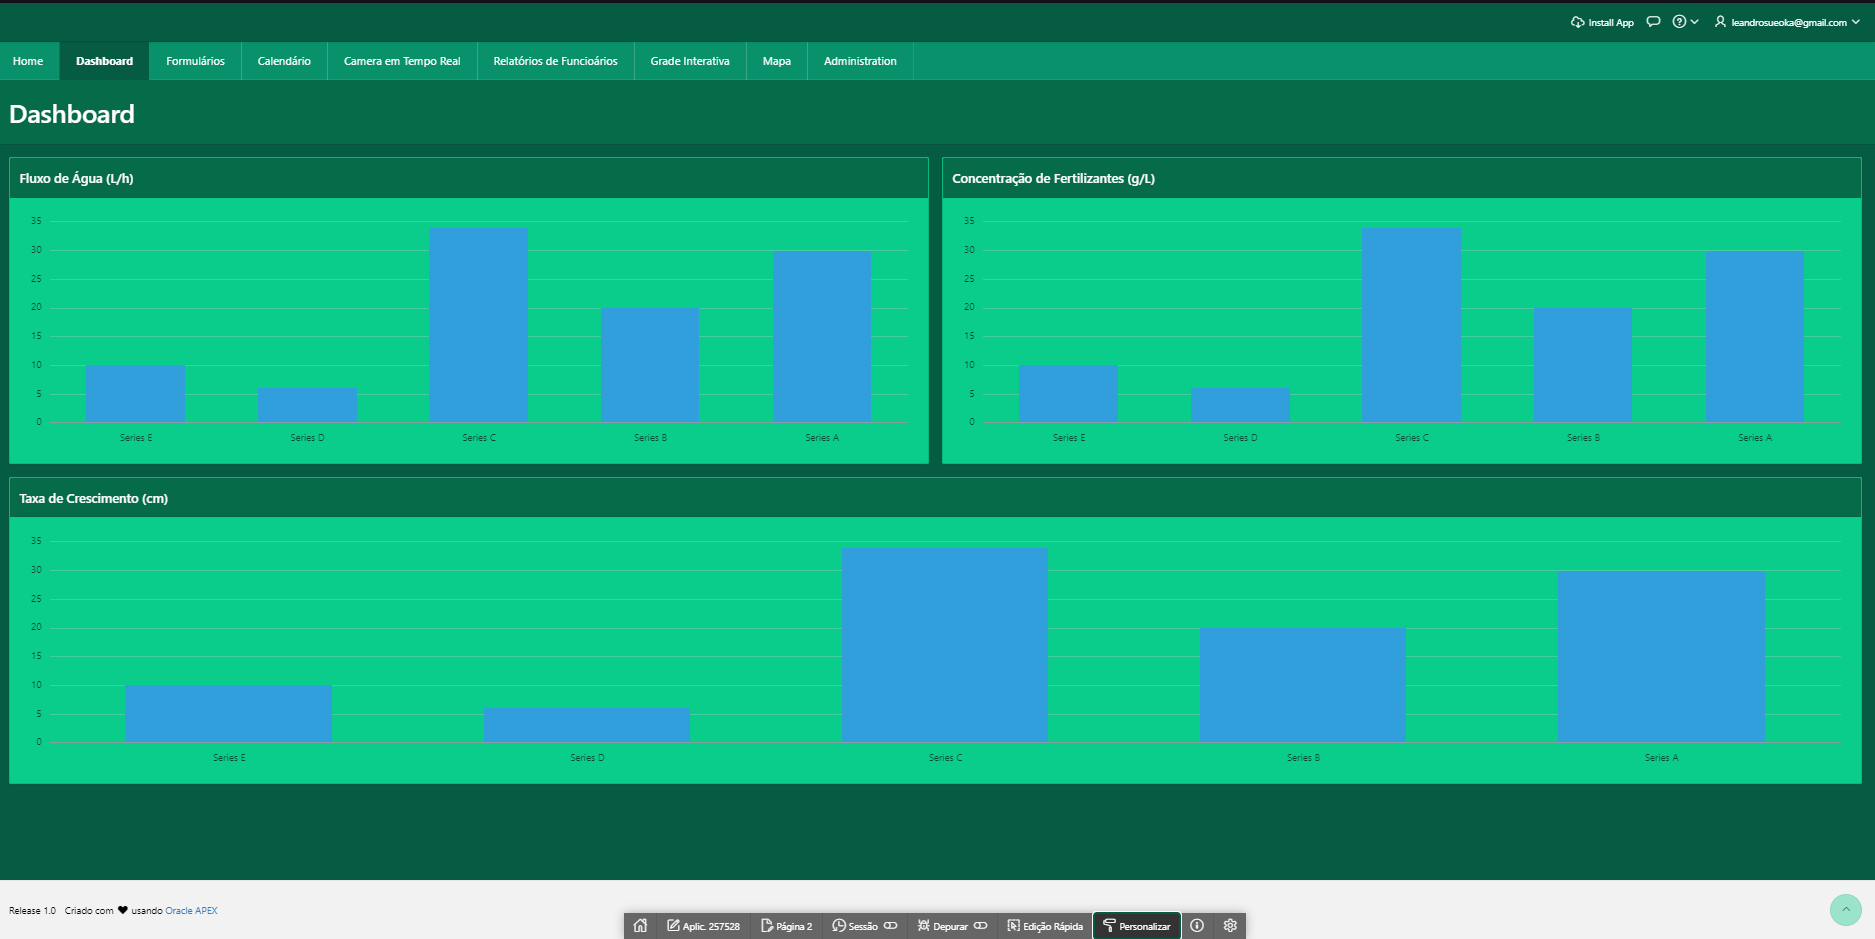
\includegraphics[scale=0.2]{Illustrations/Tela_dashboard.png}
\SourceOrNote{Autoria Própria (2024)}
\end{figure}

Temos uma tela de dashboards com os indicadores apresentando dados históricos de taxa de crescimento, fluxo de água e concentração do fertilizante. São gráficos baseados em Oracle Jet, personalizáveis pelo adminitrador do sistema.

\begin{figure}[!h]
\centering
\caption{Tela de relatórios}
\label{fig:picture21}
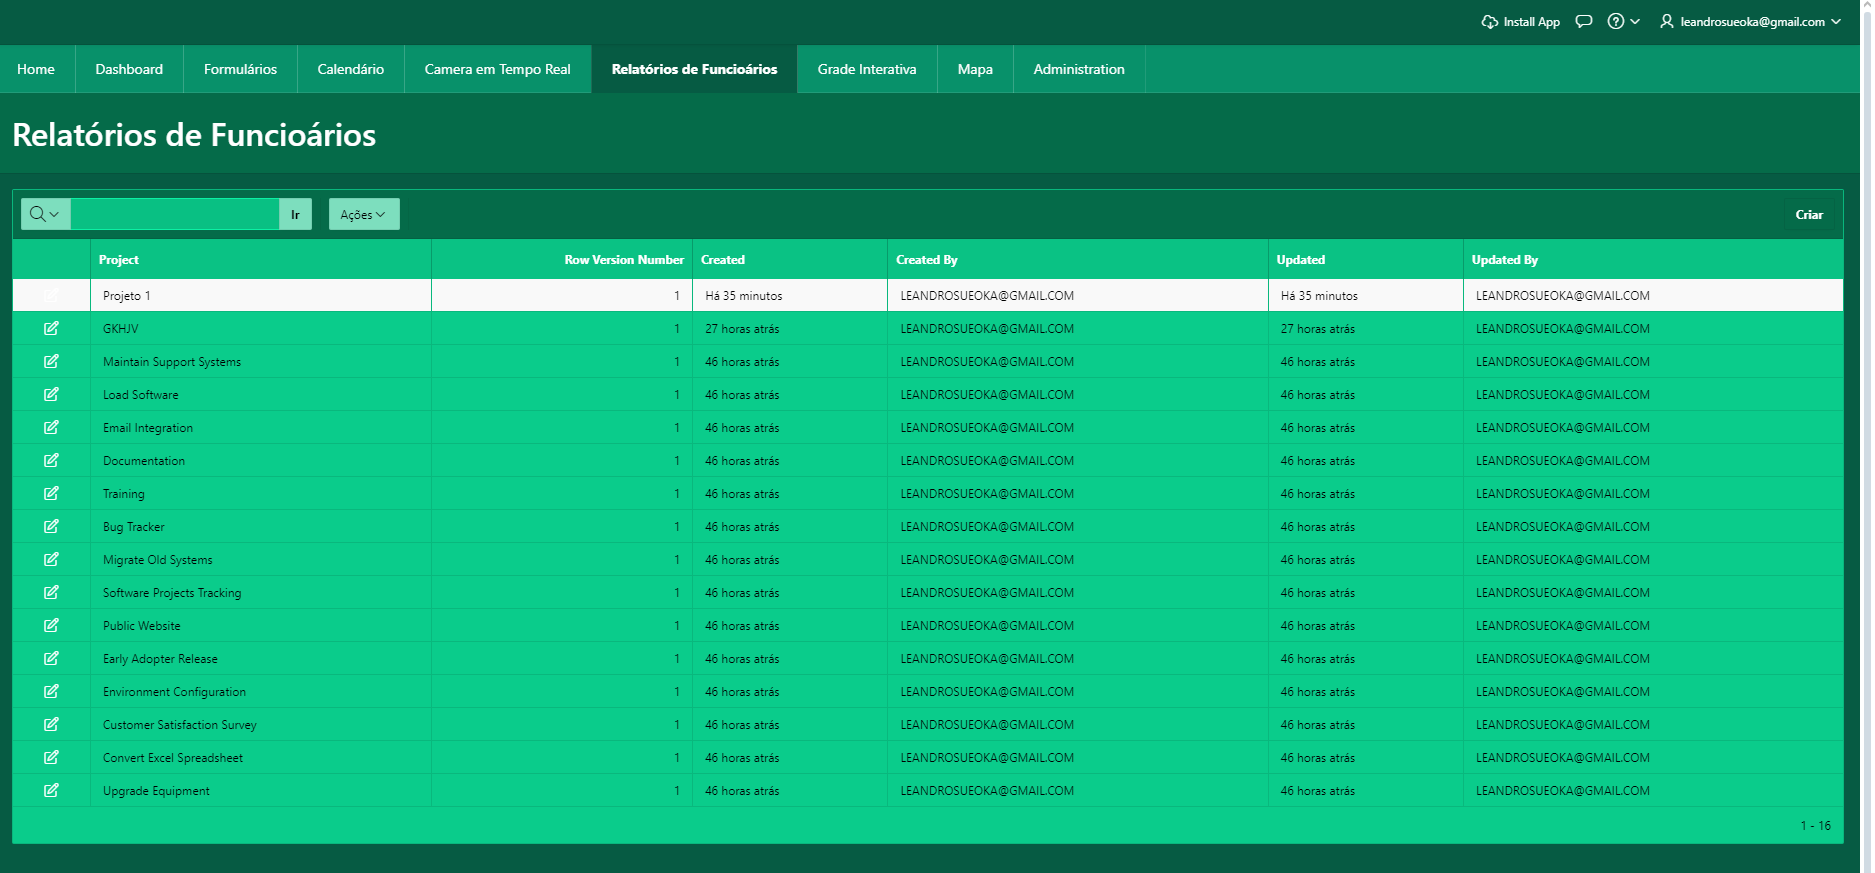
\includegraphics[scale=0.2]{Illustrations/Tela_relatorios_func.png}
\SourceOrNote{Autoria Própria (2024)}
\end{figure}

Temos uma tela de relatórios onde o usuário pode extrair informações mais detalhadas do banco de dados do sistema. Existe um campo de busca onde é possível verificar uma informação específica no banco de dados.

\begin{figure}[!h]
\centering
\caption{Grade interativa}
\label{fig:picture22}
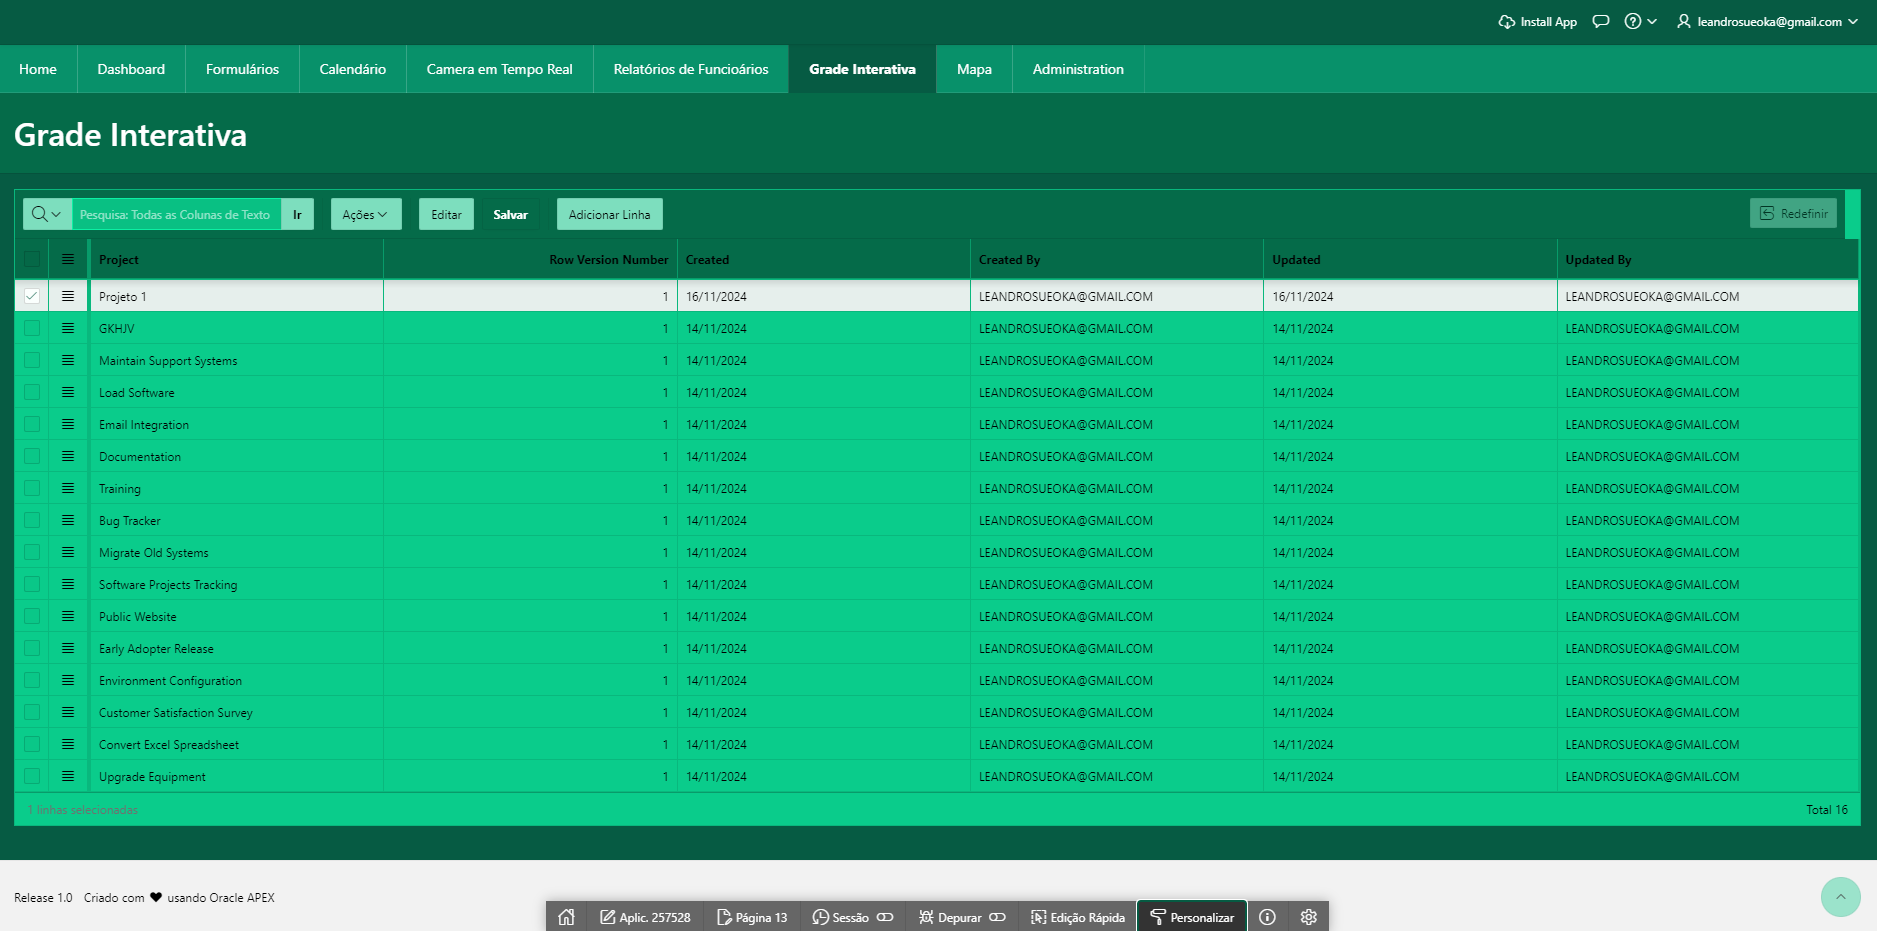
\includegraphics[scale=0.2]{Illustrations/Tela_grade_interativa.png}
\SourceOrNote{Autoria Própria (2024)}
\end{figure}
    
Temos uma tela de grade interativa que exibe diversas informações presentes no banco de dados. Estas informações podem ser filtradas diretamente na tela de forma simples e intuitiva.
\clearpage
\begin{figure}[!h]
\centering
\caption{Tela de mapa}
\label{fig:picture23}
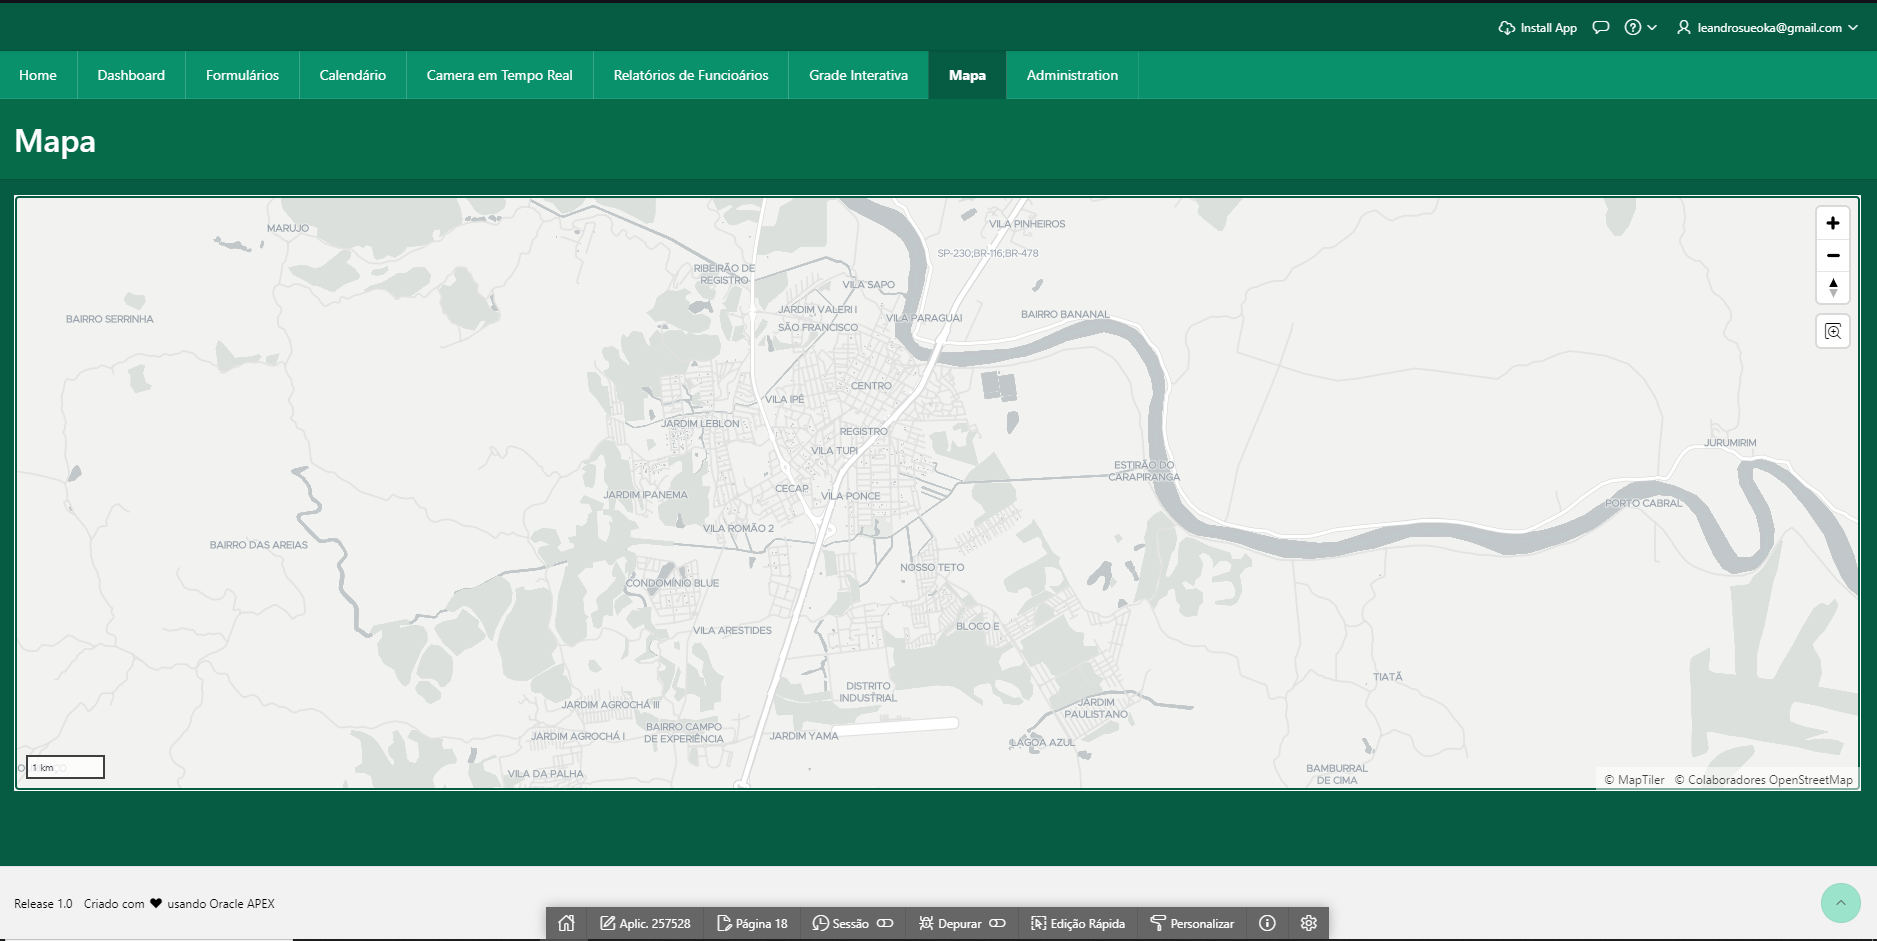
\includegraphics[scale=0.2]{Illustrations/Tela_mapa.png}
\SourceOrNote{Autoria Própria (2024)}
\end{figure}
        
O sistema conta também com uma tela de mapa, que exibe o local onde a(s) fazenda(s) vertical(is) estão situadas.

\begin{figure}[!h]
\centering
\caption{Tela de administração}
\label{fig:picture24}
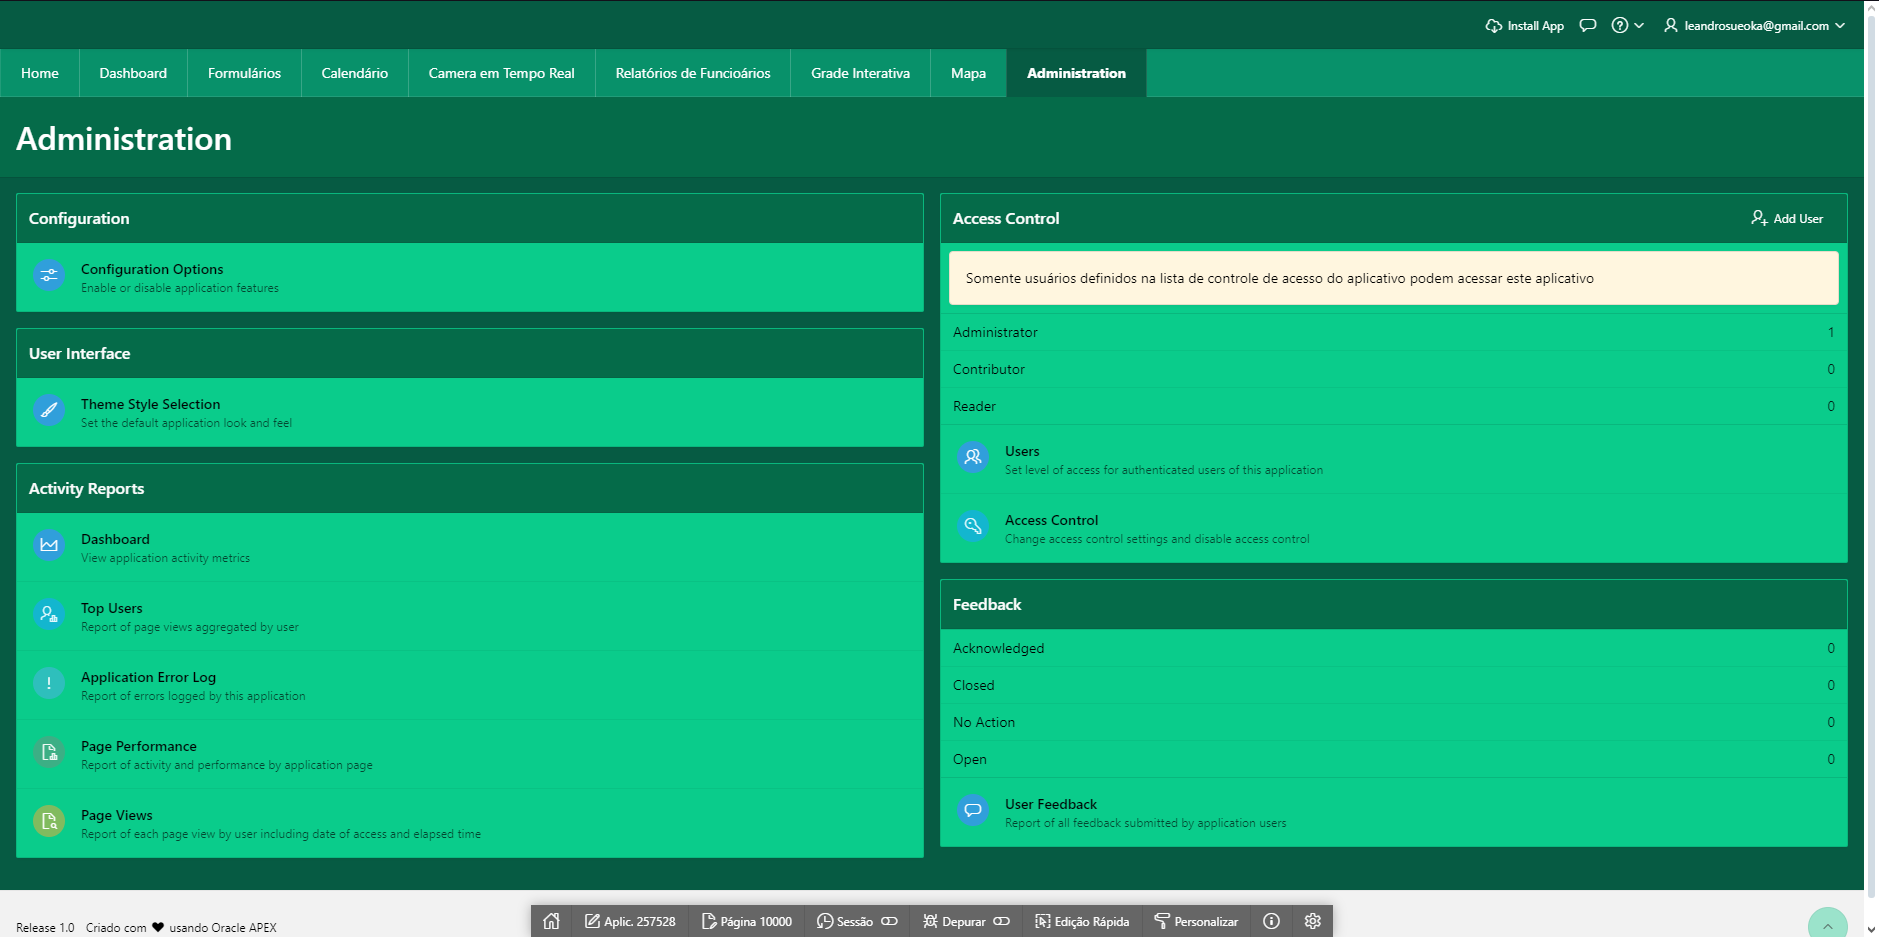
\includegraphics[scale=0.2]{Illustrations/Tela_adiministracao.png}
\SourceOrNote{Autoria Própria (2024)}
\end{figure}
            
O sistema conta com uma tela de administração onde o usuário pode personalizar algumas opções da aplicação (configuração e opções, seleção de tema, relatórios de atividades envolvendo dashboards, páginas visualizadas por usuário, log de erros, performance da página, visualizações, controle de acesso e opções de feedback referente o aplicativo).

\begin{figure}[!h]
\centering
\caption{Tela de calendario}
\label{fig:picture25}
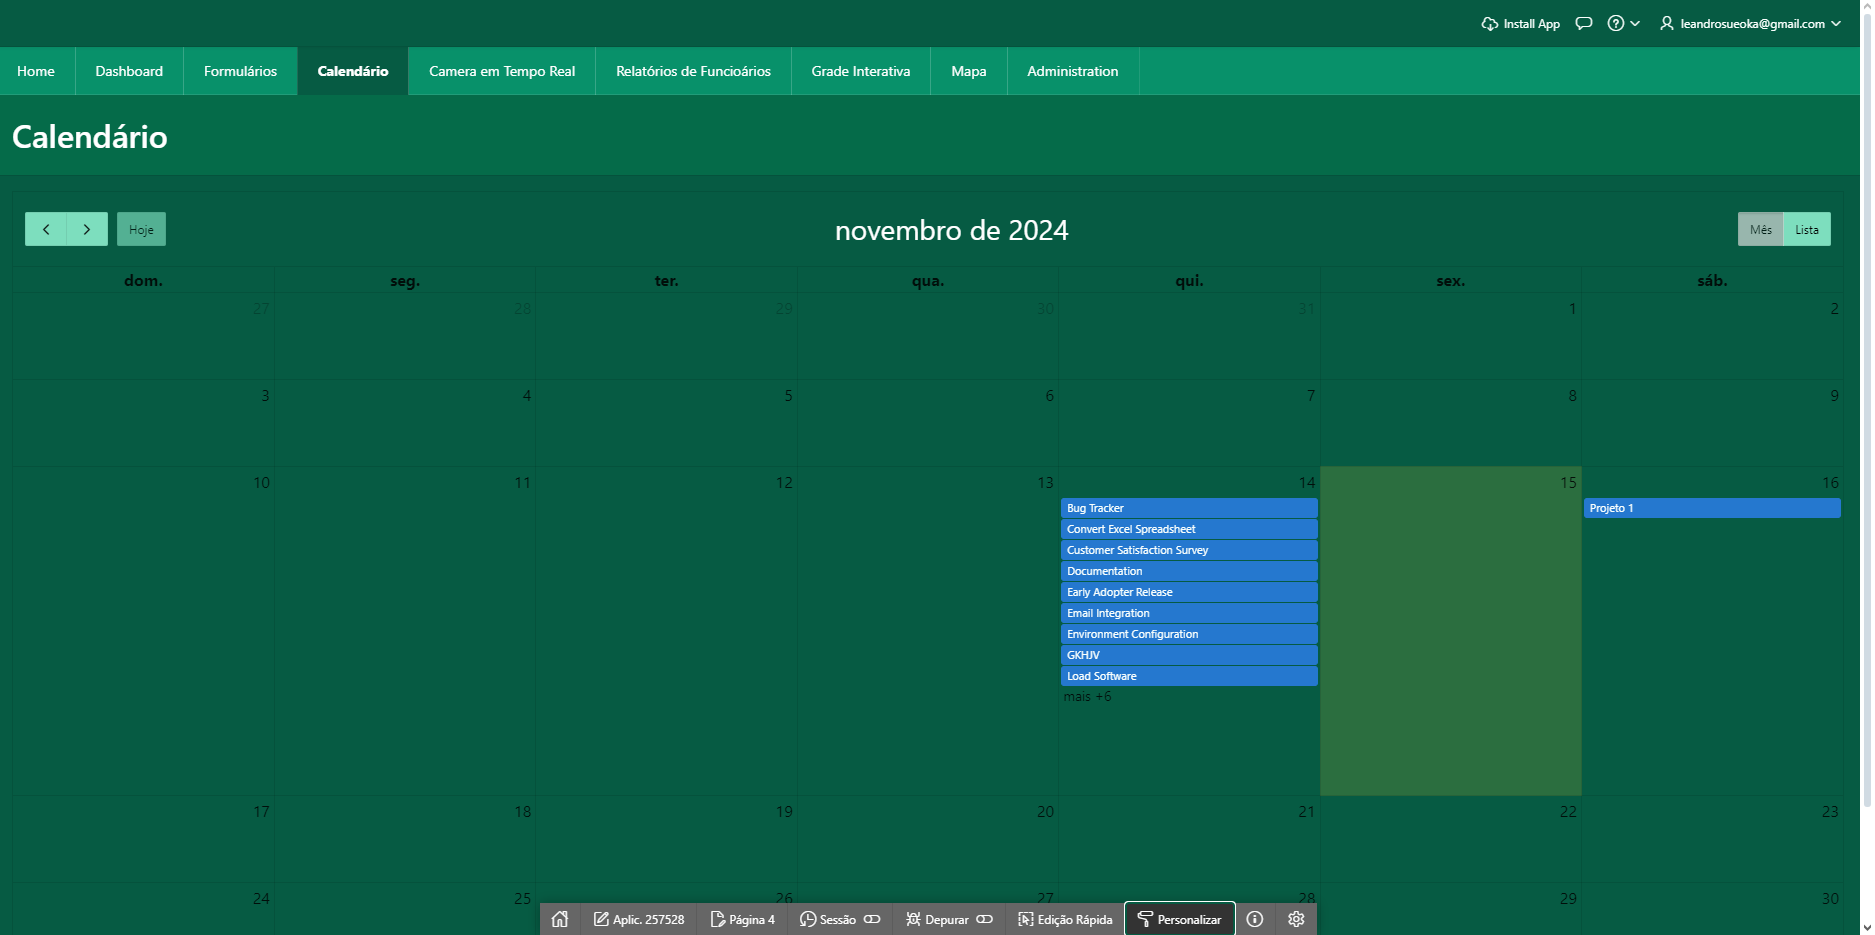
\includegraphics[scale=0.2]{Illustrations/Tela_calendario.png}
\SourceOrNote{Autoria Própria (2024)}
\end{figure}
                
O sistema também conta com uma tela de calendário, onde o usuário pode realizar quaisquer tipos de anotações referentes a fazenda vertical em função do tempo.

\subsection*{SITE}

Com o intuito de apresentar o projeto e a equipe envolvida foi desenvolvido um site.

\begin{figure}[!h]
\centering
\caption{Site}
\label{fig:picture26}
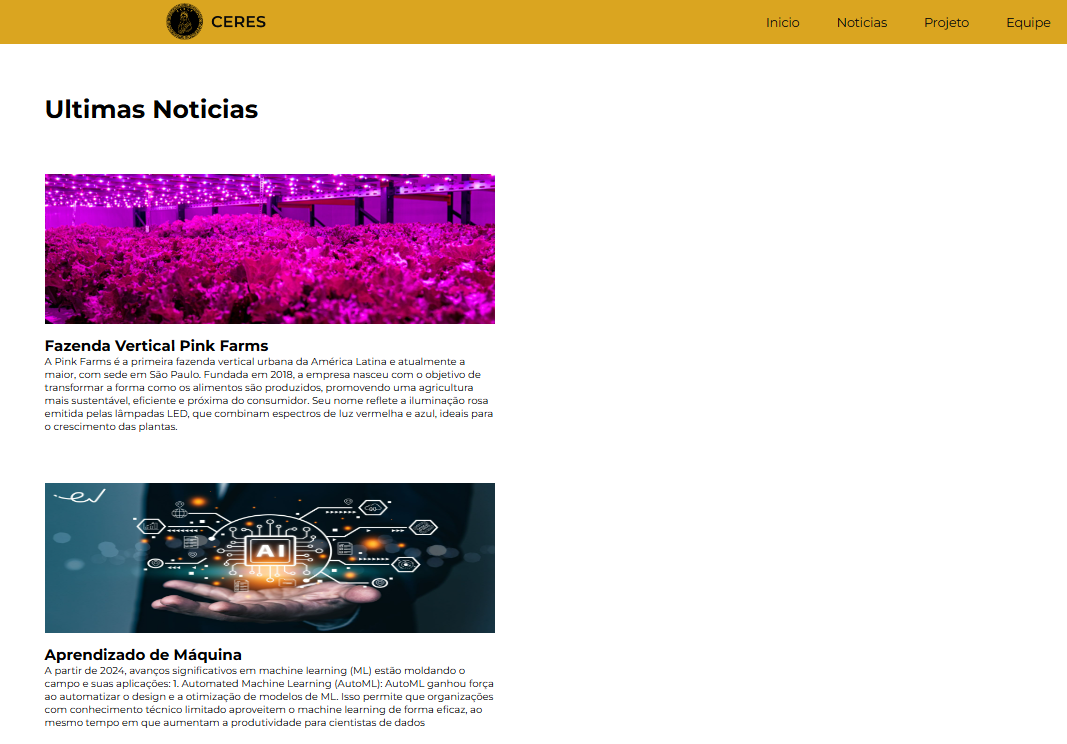
\includegraphics[scale=0.5]{Illustrations/site.png}
\SourceOrNote{Autoria Própria (2024)}
\end{figure}
O site tem uma página e foi desenvolvido em HTML. Na barra superior conta com um menu com quatro botões (Início, notícias, Projeto e equipe). Cada é um atalho para o trecho designado no site. 

\section*{CONCLUSÃO}\label{sect:conclusao}

No artigo de Phukan et al (2022) foi desenvolvido um projeto de hidroponia utilizando IoT e Machine Learning. Embora o artigo seja voltado para a produção de tomates e em solo, os autores obtiveram resultados promissores e abriram possibilidades para produção em larga escala e mais variedades de culturas hidropônicas. O artigo de Suresh et al (2024) baseou-se em uma fazenda hidropônica e um sistema de IoT. Embora tenha alguma semelhança, o autor não utilizou IA para automatizar e atingir os resultados obtidos.
Por sua vez o artigo de Saraswathy et al (2020) tem uma premissa muito parecida com o nosso, integrando IA e IoT em uma fazenda hidropônica. Os autores não indicam qual a variedade hidropônica foi cultivada, também não utilizaram um aplicativo móvel para controle e monitoramento. Em contrapartida, utilizaram-se de sensores para automatizar os controles de umidade, ph, temperatura, controle de luz e fluxo de água. Os autores finalizaram seu trabalho com a possibilidade de expandir os controles automatizados para toda a produção do local de estudo, oferecendo assim grandes possibilidades ao nosso trabalho. 
Os próximos passos para o nosso trabalho são o aprimoramento do projeto para aplicação em campo.

\printbibliography

%% Elementos pós-textuais (opcionais): Apêndice e Anexo
%Caso for utilizar, basta retirar o símbolo de % na frente do comando
%%%%% Elementos pós-textuais
%%
%% Glossário, apêndices, anexos e índice remissivo (opcionais).

%% Apêndices
\begin{Appendix}

\section{Título de Apêndice}%
\label{sect:apx-a1}

Exemplo de apêndice (\Cref{sect:apx-a1}) em uma seção de \nameref{sect:appendix}.

\subsection{Título de Seção Secundária de Apêndice}%
\label{ssect:apx-a2}

Exemplo de seção secundária de apêndice (\Cref{ssect:apx-a2}).

\subsubsection{Título de Seção Terciária de Apêndice}%
\label{sssect:apx-a3}

Exemplo de seção terciária de apêndice (\Cref{sssect:apx-a3}).

\paragraph{Título de seção quaternária de Apêndice}%
\label{prgh:apx-a4}

Exemplo de seção quaternária de apêndice (\Cref{prgh:apx-a4}).

\subparagraph{Título de seção quinária de Apêndice}%
\label{sprgh:apx-a5}

Exemplo de seção quinária de apêndice (\Cref{sprgh:apx-a5}).

\end{Appendix}

%% Anexos
\begin{Annex}

\section{Título de Anexo}%
\label{sect:anx-a1}

Exemplo de anexo (\Cref{sect:anx-a1}) em uma seção de \nameref{sect:annex}.

\subsection{Título de Seção Secundária de Anexo}%
\label{ssect:anx-a2}

Exemplo de seção secundária de anexo (\Cref{ssect:anx-a2}).

\subsubsection{Título de Seção Terciária de Anexo}%
\label{sssect:anx-a3}

Exemplo de seção terciária de anexo (\Cref{sssect:anx-a3}).

\paragraph{Título de seção quaternária de Anexo}%
\label{prgh:anx-a4}

Exemplo de seção quaternária de anexo (\Cref{prgh:anx-a4}).

\subparagraph{Título de seção quinária de Anexo}%
\label{sprgh:anx-a5}

Exemplo de seção quinária de anexo (\Cref{sprgh:anx-a5}).

\end{Annex}

%% Índice remissivo
\printindex%


%% Fim do documento
\end{document}